\documentclass[conference]{IEEEtran}
\IEEEoverridecommandlockouts
\usepackage{cite}
\usepackage{amsmath,amssymb,amsfonts}
\usepackage{algorithmic}
\usepackage{graphicx}
\usepackage{textcomp}
\usepackage{xcolor}
\usepackage{booktabs}
\usepackage{multirow}
\usepackage{url}
\usepackage{hyperref}
\hypersetup{colorlinks=true, linkcolor=blue, citecolor=blue, urlcolor=blue}

\def\BibTeX{{\rm B\kern-.05em{\sc i\kern-.025em b}\kern-.08em
    T\kern-.1667em\lower.7ex\hbox{E}\kern-.125emX}}

\begin{document}

\title{Neural Machine Translation for Sourashtra: A Progressive Approach from Character-Level Seq2Seq to Byte-Level Transformers with Cross-Lingual Transfer}

\author{
\IEEEauthorblockN{J. K. Pranav Aditya}
\IEEEauthorblockA{
\textit{Department of Computational Intelligence} \\
\textit{SRM Institute of Science and Technology} \\
Kattankulathur, India \\
ja6600@srmist.edu.in
}
\and
\IEEEauthorblockN{E. Poongothai}
\IEEEauthorblockA{
\textit{Department of Computational Intelligence} \\
\textit{SRM Institute of Science and Technology} \\
Kattankulathur, India \\
poongote@srmist.edu.in
}
}

\maketitle


\begin{abstract}
Low-resource languages present a persistent challenge for neural machine translation because large parallel corpora are typically unavailable. Sourashtra, an endangered Indo-Aryan language spoken by roughly half a million people in southern India, lacks any publicly available NMT system. In this paper, we describe a progressive research effort to build a Sourashtra-to-English translation system, beginning with a character-level GRU encoder-decoder and ending with a byte-level Transformer architecture. Our work proceeds through five model generations: (V1) a bidirectional GRU with Bahdanau attention trained at the character level, (V2) a custom Transformer with BPE subword tokenization, (V3) fine-tuning the pre-trained T5-small model, (V4) a multilingual extension that incorporates Tamil cross-lingual transfer, and (V5) fine-tuning ByT5-small, a byte-level Transformer that removes the subword vocabulary bottleneck entirely. We further introduce a hybrid inference strategy that combines neural predictions with an enhanced retrieval mechanism based on Levenshtein distance, Jaccard similarity, and prefix matching. Our best system, V5~Hybrid, reaches 9.61\% exact-match accuracy on a held-out test set of 1,914 word pairs, representing a 22.9-fold improvement over the V1 baseline. We also present a web application that provides real-time dictionary-based translation between English, Tamil, and Sourashtra, rendering output in the native Saurashtra Unicode script. All code, data, and trained models are made available for future research.
\end{abstract}

\begin{IEEEkeywords}
neural machine translation, low-resource languages, Sourashtra, byte-level Transformer, cross-lingual transfer, endangered language preservation
\end{IEEEkeywords}

% ═══════════════════════════════════════════════════════════
\section{Introduction}
% ═══════════════════════════════════════════════════════════

Machine translation has made remarkable progress in recent years, yet the benefits remain unevenly distributed. While high-resource language pairs such as English--French or English--Chinese enjoy near-human fluency from modern Transformer-based systems~\cite{vaswani2017attention}, thousands of languages around the world have little or no parallel data, making them effectively invisible to state-of-the-art NMT research.

Sourashtra is one such language. It belongs to the Indo-Aryan branch of the Indo-European family and is spoken by approximately 500,000 people, mostly in the Madurai district of Tamil Nadu, India~\cite{ethnologue2023}. The language has its own script---Saurashtra, encoded in Unicode 5.1 (block U+A880--U+A8DF)---and a rich literary tradition, but it is classified as ``definitely endangered'' by UNESCO. No publicly accessible NMT system currently exists for Sourashtra, and the only available parallel data takes the form of a digitized community dictionary containing roughly 12,700 word-level entries~\cite{sourashtra_dict}.

Building a translation system under these constraints demands creative solutions. In this paper, we report a progressive, five-generation research effort designed to push translation quality upward despite the extremely limited training data. Our contributions are as follows:

\begin{enumerate}
    \item We construct and release a cleaned parallel corpus of 12,758 Sourashtra--English word pairs organized into 106 semantic categories, supplemented by Tamil equivalents and native-script annotations.
    \item We benchmark five distinct neural architectures, from a simple character-level GRU to a 300M-parameter byte-level Transformer, and document the gains achieved at each stage.
    \item We propose a hybrid inference strategy that fuses neural model outputs with a retrieval system based on three complementary similarity signals, raising exact-match accuracy to 9.61\%.
    \item We develop a publicly accessible web application that translates English and Tamil queries into Sourashtra, displaying results in the native Saurashtra script.
\end{enumerate}

The remainder of the paper is organized as follows. Section~\ref{sec:related} reviews related work. Section~\ref{sec:dataset} discusses the dataset and the preprocessing technique used. Section~\ref{sec:models} shows the five model generations, i.e., V1 to V5 along with model architectures . Section~\ref{sec:hybrid} explains about the hybrid retrieval system V5. Section~\ref{sec:experiments} details about our experimental setup, and Section~\ref{sec:results} analyzes results with the comparison. Section~\ref{sec:webapp} covers the simple web application . Section~\ref{sec:conclusion} concludes with results and future Works.

% ═══════════════════════════════════════════════════════════
\section{Related Work}\label{sec:related}
% ═══════════════════════════════════════════════════════════

\subsection{Low-Resource Neural Machine Translation}

The research indicates an increasing interest in neural
machine translation systems that perform in low-resource con-
ditions. The research proves its effectiveness~\cite{liu2020mbart, xue2021mt5} via transfer learning from the models that are pre-trained in multiple languages,while data augmentation techniques, i.e., back translation~\cite{sennrich2016backtranslation} and
transferr~\cite{neubig2018rapid}, allow researchers to develop translation systems in conditions of insufficient data. The parent model that Zoph et
al. used for training their high-resource language was effective
for fine-tuning their low-resource language, as it produced
substantial results with merely a few thousand sentence pairs.

\subsection{Byte-Level and Character-Level Models}
Subword tokenization techniques BPE~\cite{sennrich2016bpe} and Sentence Piece~\cite{kudo2018sentencepiece}  are considered standard for modern neural machine translation systems. The systems are not able to work on scripts for which there is insufficient training data to construct the required vocabulary. The problem~\cite{lee2017fully} is solved by using character-level techniques. Byte-level models, which include ByT5~\cite{xue2022byt5}, are able to achieve comparable performance without relying on any vocabulary system. ByT5 works directly on raw UTF-8 byte sequences, which helps to avoid issues related to unknown tokens and script tokenizer development.


\subsection{Endangered Language Technology}
The development of natural language processing tools for endangered languages has been done in three areas, namely, indigenous Australian languages~\cite{foley2018building}, speech recognition, and Inuktitut~\cite{micher2017improving} morphological analysis and machine translation development for Welsh, Irish, and Scottish Gaelic~\cite{dowling2020smt} languages. The research team found out that there had been no previous publications on the use of neural machine translation for the study of the Sourashtra language.

% ═══════════════════════════════════════════════════════════
\section{Dataset}\label{sec:dataset}
% ═══════════════════════════════════════════════════════════

\subsection{Data Collection and Preparation}
We have chosen the community-based Sourashtra dictionary project~\cite{sourashtra_dict}  as our primary source of data. The reason for choosing this project was not coincidental. The project offers a unified form of all Sourashtra word entries, as it includes their original script as well as their romanization form, along with matching English and Tamil translations. The system offers different layers, which help us verify their meanings, pronunciation, and usage while maintaining standards for writing systems. The system offers a complete linguistic system along with translations, which helps researchers understand different writing systems and languages.We cleaned the raw data by removing duplicates, normalizing whitespace, and discarding entries that lacked either a source or a target field. The resulting corpus contains 12,758 unique word pairs.

Each entry in the corpus consists of five fields: (1) the word in native Saurashtra script, (2) a Latin-alphabet romanized form, (3) an English meaning, (4) a Tamil meaning, and (5) a semantic category label drawn from a set of 106 categories such as \textit{Body-Parts}, \textit{Animals}, \textit{Food}, \textit{Kinship}, and \textit{Colors}.

\subsection{Data Splits}

All experiments in this work use a fixed random split (seed~=~42) of the base Sourashtra--English pairs: 9,568 pairs for training (75\%), 1,276 for validation (10\%), and 1,914 for testing (15\%). The split was stratified by category where possible. Augmentation strategies differ across model versions, as described in Section~\ref{sec:models}.

\subsection{Augmentation}

Starting with V3, we augmented the training data with 1,724 English sentence-level pairs mined from an example-sentence sub-corpus, bringing the V3 training set to 11,292 examples. V4 added 9,568 Tamil--English pairs derived from the same dictionary entries, raising the count to 20,860. V5 further expanded this by including 1,725 Tamil sentence-level pairs, yielding 22,585 total training examples---a 2.36$\times$ augmentation ratio relative to the base split.

Table~\ref{tab:dataset} summarizes these figures.

\begin{table}[htbp]
\centering
\caption{Dataset Statistics Across Model Versions}
\label{tab:dataset}
\begin{tabular}{lr}
\toprule
\textbf{Statistic} & \textbf{Value} \\
\midrule
Total unique word pairs & 12,758 \\
Base training set (SR$\rightarrow$EN) & 9,568 \\
Validation set & 1,276 \\
Test set & 1,914 \\
Semantic categories & 106 \\
\midrule
V3 training (+ EN sentences) & 11,292 \\
V4 training (+ Tamil pairs) & 20,860 \\
V5 training (+ Tamil sentences) & 22,585 \\
\bottomrule
\end{tabular}
\end{table}

% ═══════════════════════════════════════════════════════════
\section{Model Architectures}\label{sec:models}
% ═══════════════════════════════════════════════════════════

We developed five successive model versions. Each generation was designed to address specific weaknesses observed in its predecessor.

\subsection{V1: Character-Level GRU with Attention}

Our first system uses a bidirectional GRU encoder paired with a GRU decoder connected through Bahdanau additive attention~\cite{bahdanau2015attention}. Both the encoder and decoder have 2 layers with a hidden dimension of 256. The embedding dimension is 128, and a bridge layer projects the encoder's final states into the decoder's initial hidden state. The source vocabulary consists of 38 unique characters, while the target vocabulary contains 55.

We used Adam with a learning rate of $10^{-3}$ and ReduceLROnPlateau scheduling (patience~5, factor~0.5). Teacher forcing was annealed from 1.0 to 0.3 at a rate of 0.97 per epoch. Gradient clipping was set to 1.0, and dropout to 0.3. Training ran for 32 epochs at batch size 128 with early stopping (patience~15).

With this specific system configuration, the model has attained and achived an exact-match accuracy of just 0.42\%. This result underscores the inherent difficulty of the task. The relationship between Sourashtra romanized forms and their corresponding English spellings is marked by substantial character-level irregularity, with few stable or predictable alignment patterns. As a result, the limited capacity of the small GRU-based architecture appears insufficient to model this variability effectively. In particular, the network lacks the representational depth needed to learn robust alignment mappings from the available training data.

\subsection{V2: Transformer with BPE Tokenization}

The development of Version 2 (V2) offers the benefits of advanced functionality through its implementation of the standard "Transformer" encoder-decoder architecture, including three layers of the ~\cite{vaswani2017attention} encoder and three layers of the decoder, as well as eight attention heads and $d_\text{model}$~=~256  dimensions for the model and 512 dimensions for the feed-forward network.

It also offers the ability to develop separate subword vocabularies through the implementation of the "SentencePiece",  algorithm~\cite{kudo2018sentencepiece}:, resulting in 1000 tokens for the source and 2000 tokens for the target, as well as character operations. It offers the ability for the model to recognize subword patterns, which display stable patterns of behavior, as well as the ability to recognize rare patterns of language.

The training process implemented the use of a linear warmup schedule during the initial 500 steps, after which it used the cosine decay function, resulting in the highest learning rate at $5 \times 10^{-4}$. It also implemented the use of 0.1 as the label smoothing, which helped the model generalize better. The process of training the model was complete after 48 epochs, with the implementation of a batch size of 128.

The implementation of the "beam search" decoding method, with the use of a beam width of 5, provided better results compared to the implementation of the "greedy" decoding method during the process of inferring the model. The exact match accuracy improved from 2.04\% with the "greedy" method to 2.56\% with the "beam search" method. The total time required for the training process of the system configuration took approximately 7 minutes.

The shift from characters to subwords and from RNNs to Transformers produced a 6.1$\times$ improvement over V1, but accuracy remained low.

\subsection{V3: Fine-Tuning T5-small}

Recognizing that our dataset is too small to train a Transformer from scratch, V3 leverages transfer learning by fine-tuning T5-small~\cite{raffel2020t5}, a 60M-parameter pre-trained encoder-decoder. T5 was originally trained on the Colossal Clean Crawled Corpus (C4), giving it strong English language understanding.

We fed source-side inputs with a category prefix (e.g., \texttt{``translate Body-Parts: angam''}) to provide the model with domain context. Training used Adafactor at $10^{-3}$, cosine scheduling, effective batch size of 64 (32~$\times$~2 gradient accumulation), and FP16 mixed precision. We also augmented the training data with 1,724 corpus sentence pairs.

V3 achieved 6.01\% exact-match accuracy---a 14.3$\times$ improvement over V1 and a clear demonstration that pre-training compensates substantially for small data size. BLEU reached 4.72 and chrF reached 18.47.

\subsection{V4: Cross-Lingual Transfer with Tamil}

Sourashtra has been spoken alongside Tamil for centuries, and the two languages share Dravidian lexical influences. V4 tested whether adding Tamil--English parallel data could improve Sourashtra--English translation through cross-lingual transfer.

We retained the T5-small architecture from V3 and introduced a multi-task training scheme. Each batch contained a mixture of Sourashtra$\rightarrow$English pairs (loss weight 1.0) and Tamil$\rightarrow$English pairs (loss weight 0.8). The Tamil pairs were drawn from the same dictionary, using the Tamil meaning field as the source. This roughly doubled the training data to 20,860 examples.

Somewhat surprisingly, V4's neural exact-match accuracy dropped to 5.80\% from V3's 6.01\%. We attribute this to a mismatch between T5-small's tokenizer and Tamil text: T5 lacks native Tamil vocabulary and falls back to byte-level tokenization for non-Latin scripts, introducing noise into the shared representation space. Despite the neural regression, the combined hybrid result with retrieval improved to 7.68\% (Section~\ref{sec:hybrid}).

\subsection{V5: ByT5-small---Byte-Level Translation}

The insight from V4's failure guided V5. If the tokenizer is the bottleneck for handling multiple scripts, then a model that requires no tokenizer at all should perform better. ByT5-small~\cite{xue2022byt5} is a variant of the T5 model, which works directly on raw UTF-8 byte sequences rather than specific tokens. The system works by performing a byte-level analysis of the input, which eliminates the need for a specific vocabulary. The model is able to work on different writing systems without the need for token-based systems for character representation. It has 300M parameters arranged in 12 encoder layers and 4 decoder layers with $d_\text{model}$~=~1,472.

Training ByT5 on an 8~GB GPU (NVIDIA RTX 4060) required gradient checkpointing and BF16 mixed precision (FP16 produced NaN losses due to the large $d_\text{model}$). We used effective batch size 64 (16~$\times$~4 gradient accumulation), Adafactor at $10^{-3}$ with cosine scheduling and a warmup ratio of 0.06. Training ran for 20 epochs and took approximately 119 minutes.

V5 achieved 9.25\% exact-match accuracy---the highest neural-only result across all versions. BLEU reached 4.70 and chrF reached 22.32. The byte-level architecture gracefully handles both romanized Sourashtra and Tamil without any tokenization artifacts, validating our hypothesis about the vocabulary bottleneck.

% ═══════════════════════════════════════════════════════════
\section{Hybrid Inference}\label{sec:hybrid}
% ═══════════════════════════════════════════════════════════

We observed early in our experiments that a simple retrieval baseline---looking up the nearest entry in the training dictionary by string similarity---can achieve non-trivial accuracy on word-level translation. Since neural models and retrieval systems tend to make different kinds of errors, we designed a hybrid strategy that selects between the two at inference time.

\subsection{Retrieval Component}

The retrieval system computes a composite similarity score between the input word and every source entry in the training dictionary. Three signals are combined:

\begin{equation}
S(q, d) = 0.45 \cdot J_3(q, d) + 0.45 \cdot L(q, d) + 0.10 \cdot P(q, d)
\label{eq:retrieval}
\end{equation}

\noindent where $J_3$ is the Jaccard similarity over character trigram sets, $L$ is the normalized Levenshtein similarity ($1 - \text{dist}(q,d)/\max(|q|,|d|)$), and $P$ is the prefix overlap ratio. The top-scoring dictionary entry serves as the retrieval prediction.

\subsection{Fusion Strategy}

Given the neural prediction $\hat{y}_\text{neural}$ and the retrieval prediction $\hat{y}_\text{retrieval}$ with confidence score $S$, the hybrid system selects its output based on a threshold $\tau$:

\begin{equation}
\hat{y}_\text{hybrid} = \begin{cases}
\hat{y}_\text{retrieval} & \text{if } S \geq \tau \\
\hat{y}_\text{neural} & \text{otherwise}
\end{cases}
\end{equation}

The threshold $\tau$ is tuned on the validation set. For V5~Hybrid, $\tau$~=~0.70, meaning the retrieval result is used only when the dictionary match is very strong. At this threshold, only 24.1\% of test predictions come from retrieval, while 75.9\% rely on the neural model. In contrast, V4~Hybrid used $\tau$~=~0.45, drawing 59.2\% of its predictions from retrieval---a reflection of V5's much stronger neural backbone.


\begin{table}[htbp]
\centering
\caption{Hybrid System Comparison: V4 vs.\ V5}
\label{tab:hybrid}
\begin{tabular}{lrr}
\toprule
\textbf{Component} & \textbf{V4~Hybrid} & \textbf{V5~Hybrid} \\
\midrule
Neural model & T5-small (60M) & ByT5-small (300M) \\
Tokenization & Subword (BPE) & Byte-level (UTF-8) \\
Training precision & FP16 & BF16 \\
Retrieval method & Char n-gram & Jaccard+Lev+Pfx \\
Confidence threshold $\tau$ & 0.45 & 0.70 \\
Retrieval coverage & 59.2\% & 24.1\% \\
Neural coverage & 40.8\% & 75.9\% \\
\midrule
Hybrid EM accuracy & 7.68\% & \textbf{9.61\%} \\
\bottomrule
\end{tabular}
\end{table}

% ═══════════════════════════════════════════════════════════
\section{Experimental Setup}\label{sec:experiments}
% ═══════════════════════════════════════════════════════════

\subsection{Evaluation Metrics}

There are four established methods of quality evaluation of the translated content, which include specific criteria to maintain uniform and structured quality in the assessment of the translation performance.:

\begin{itemize}
    \item \textbf{Exact Match (EM) method}: The Exact Match method is based on the percentage of test predictions that exactly match the reference translation after the application of lower casing and whitespace normalization.
    \item \textbf{BLEU}~\cite{papineni2002bleu}: a precision-oriented $n$-gram overlap score.
    \item \textbf{chrF}~\cite{popovic2015chrf}: The character F-score of the chrF method provides accurate information about the tasks where complex morphological structures need to be managed.
    \item \textbf{CER}: character error rate, computed as the edit distance between the prediction and reference strings.
\end{itemize}

EM is our primary metric because our dataset consists of word-level pairs, and partial credit (as measured by BLEU or chrF) is less meaningful at this granularity.

\subsection{Hardware and Software}

All experiments were conducted on a single workstation equipped with an NVIDIA RTX~4060 GPU (8~GB VRAM), an Intel processor, and 32~GB of system RAM, running Windows~11. Models were implemented in PyTorch with Hugging~Face Transformers~\cite{wolf2020huggingface}. The web application was built with Flask and vanilla JavaScript.

% ═══════════════════════════════════════════════════════════
\section{Results and Analysis}\label{sec:results}
% ═══════════════════════════════════════════════════════════

\subsection{Overall Performance}

Table~\ref{tab:results} presents the main results across all model versions. Fig.~\ref{fig:em_comparison} visualizes the exact-match progression.

\begin{table}[htbp]
\centering
\caption{Comparative Performance Evaluation of All Sourashtra–English Translation Models}
\label{tab:results}
\begin{tabular}{lccccc}
\toprule
\textbf{Model} & \textbf{Params} & \textbf{EM (\%)} & \textbf{BLEU} & \textbf{chrF} & \textbf{Time} \\
\midrule
V1: Char-GRU & $\sim$1M & 0.42 & 0.00 & 8.81 & 22m \\
V2: Transformer+BPE & $\sim$5M & 2.56 & 0.00 & 11.78 & 7m \\
V3: T5-small & 60M & 6.01 & 4.72 & 18.47 & 36m \\
V3: Hybrid & 60M & 7.47 & 5.36 & 20.86 & -- \\
V4: T5+Tamil & 60M & 5.80 & 3.57 & 18.27 & 58m \\
V4: Hybrid & 60M & 7.68 & 5.28 & 21.01 & -- \\
V5: ByT5-small & 300M & 9.25 & 4.70 & 22.32 & 119m \\
\textbf{V5: Hybrid} & \textbf{300M} & \textbf{9.61} & \textbf{4.57} & \textbf{22.95} & -- \\
\bottomrule
\end{tabular}
\end{table}

\begin{figure}[htbp]
\centerline{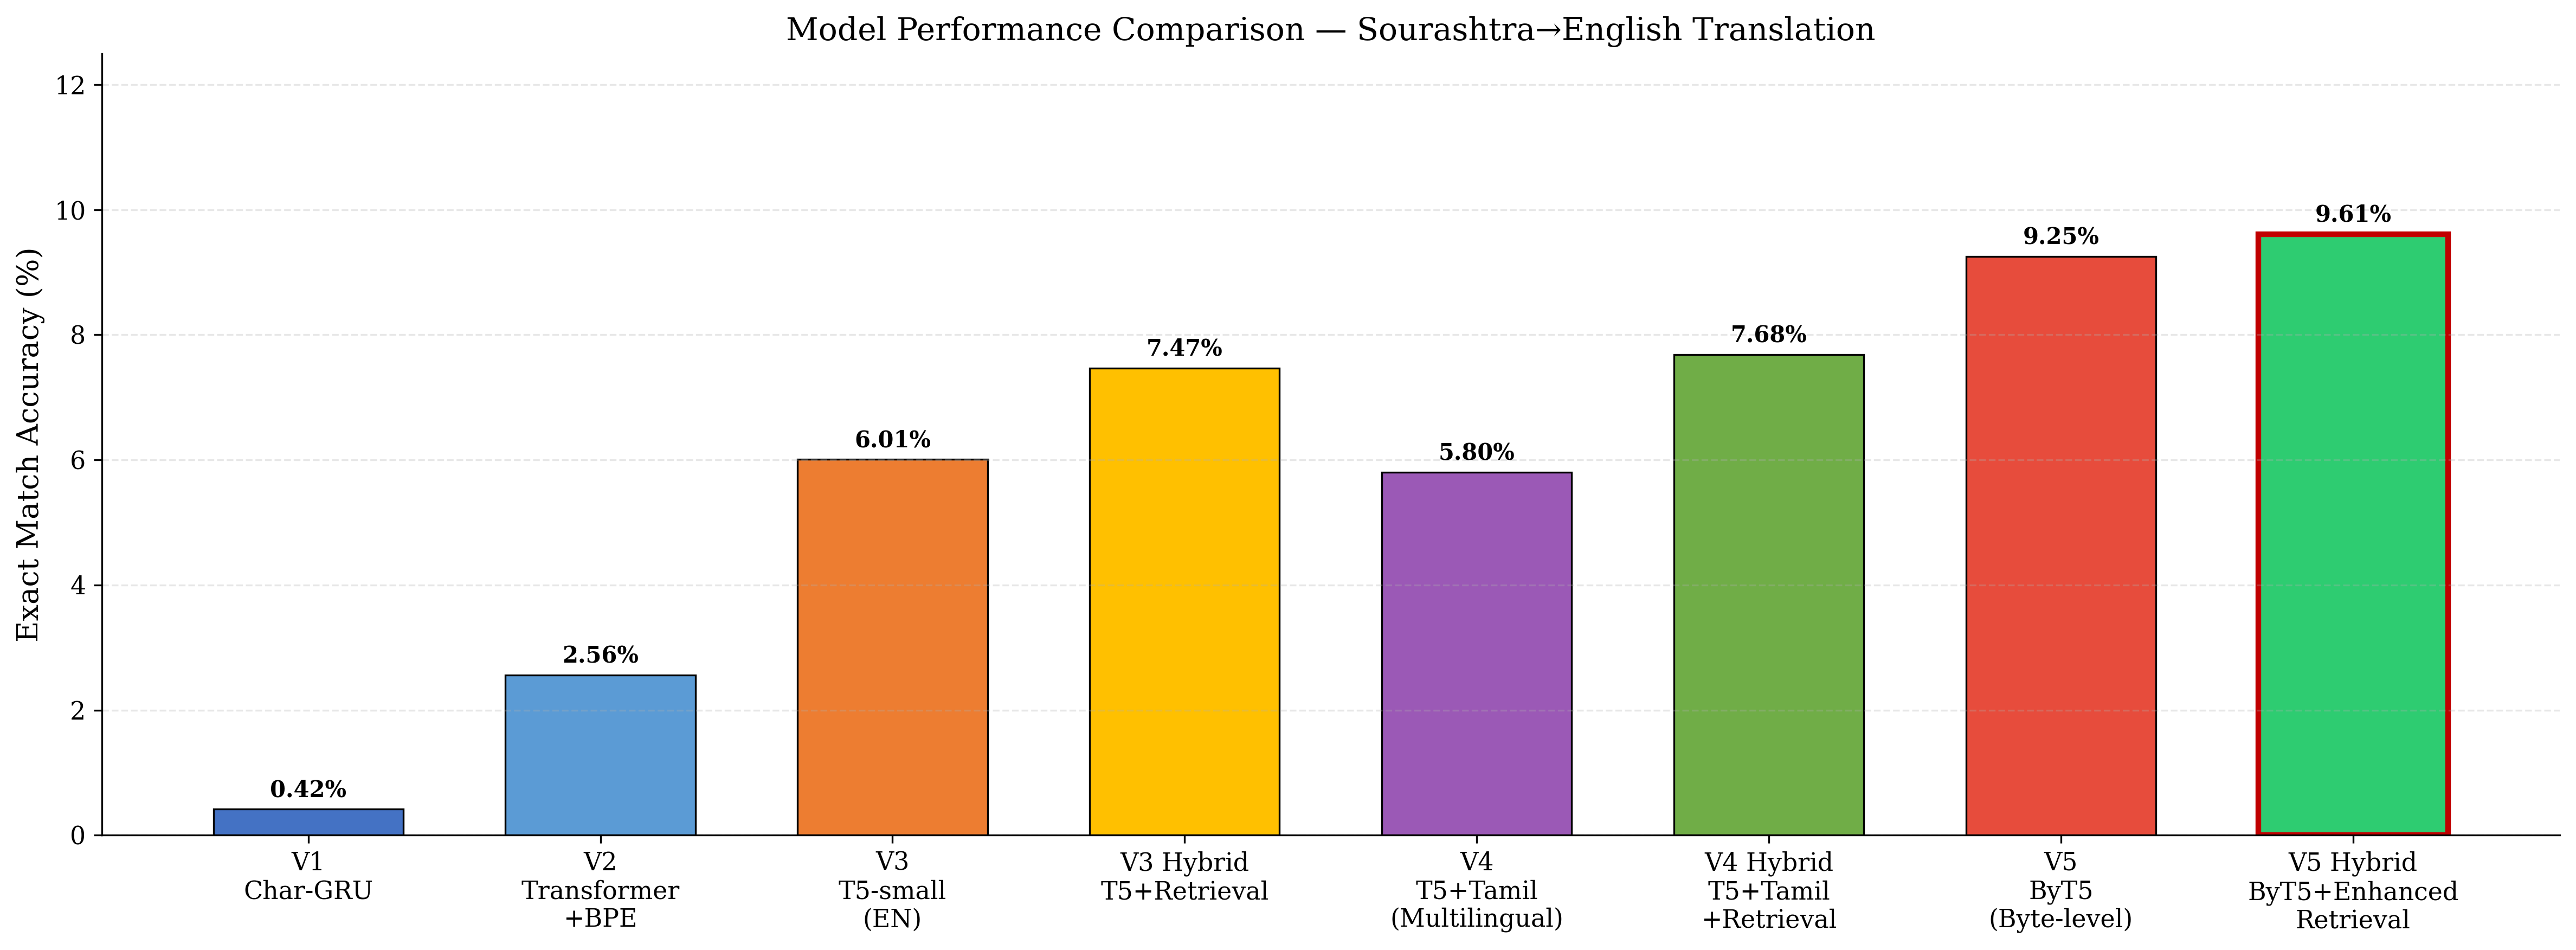
\includegraphics[width=\columnwidth]{fig1_model_comparison_em.png}}
\caption{Exact-match accuracy across all models.The V5 Hybrid system attains the best result at 9.61\%.}
\label{fig:em_comparison}
\end{figure}

Several noteworthy takeaways from these results:

\textbf{Pre-training matters more than anything else.} The jump from V2 (trained from scratch, 2.56\%) to V3 (fine-tuned T5, 6.01\%) is the single largest absolute gain in our experiments. Pre-trained language models bring general linguistic knowledge that partially compensates for the lack of Sourashtra-specific training data.

\textbf{Byte-level models resolve the tokenizer bottleneck.} V5's neural accuracy of 9.25\% surpasses all previous systems, including hybrids. ByT5's ability to process raw bytes means it handles romanized Sourashtra, English, and Tamil without relying on a vocabulary that may segment tokens incorrectly.

\textbf{Tamil cross-lingual transfer is architecture-dependent.} When added to T5-small (V4), Tamil data actually hurt neural accuracy. When added to ByT5 (V5), performance improved substantially. This confirms that tokenizer compatibility is necessary for cross-lingual benefit: T5's byte-fallback for Tamil introduced noise, whereas ByT5 processes Tamil bytes natively.

\textbf{Hybrid inference provides consistent gains.} In every version where we tested it, the hybrid system outperformed both the neural model and the retrieval baseline in isolation. For V5, the gain is modest (9.25\%~$\to$~9.61\%) because the neural model is already strong enough to warrant a high retrieval threshold ($\tau$~=~0.70).

\subsection{Architecture Comparison}

Fig.~\ref{fig:multi_metric} presents a multi-metric comparison across BLEU, chrF, and EM. The chrF metric, which measures character-level overlap, shows the steadiest improvement across generations, rising from 8.81 (V1) to 22.95 (V5~Hybrid). This indicates that even when translations are not exact matches, later models produce outputs that are orthographically containing exact matches.

\begin{figure}[htbp]
\centerline{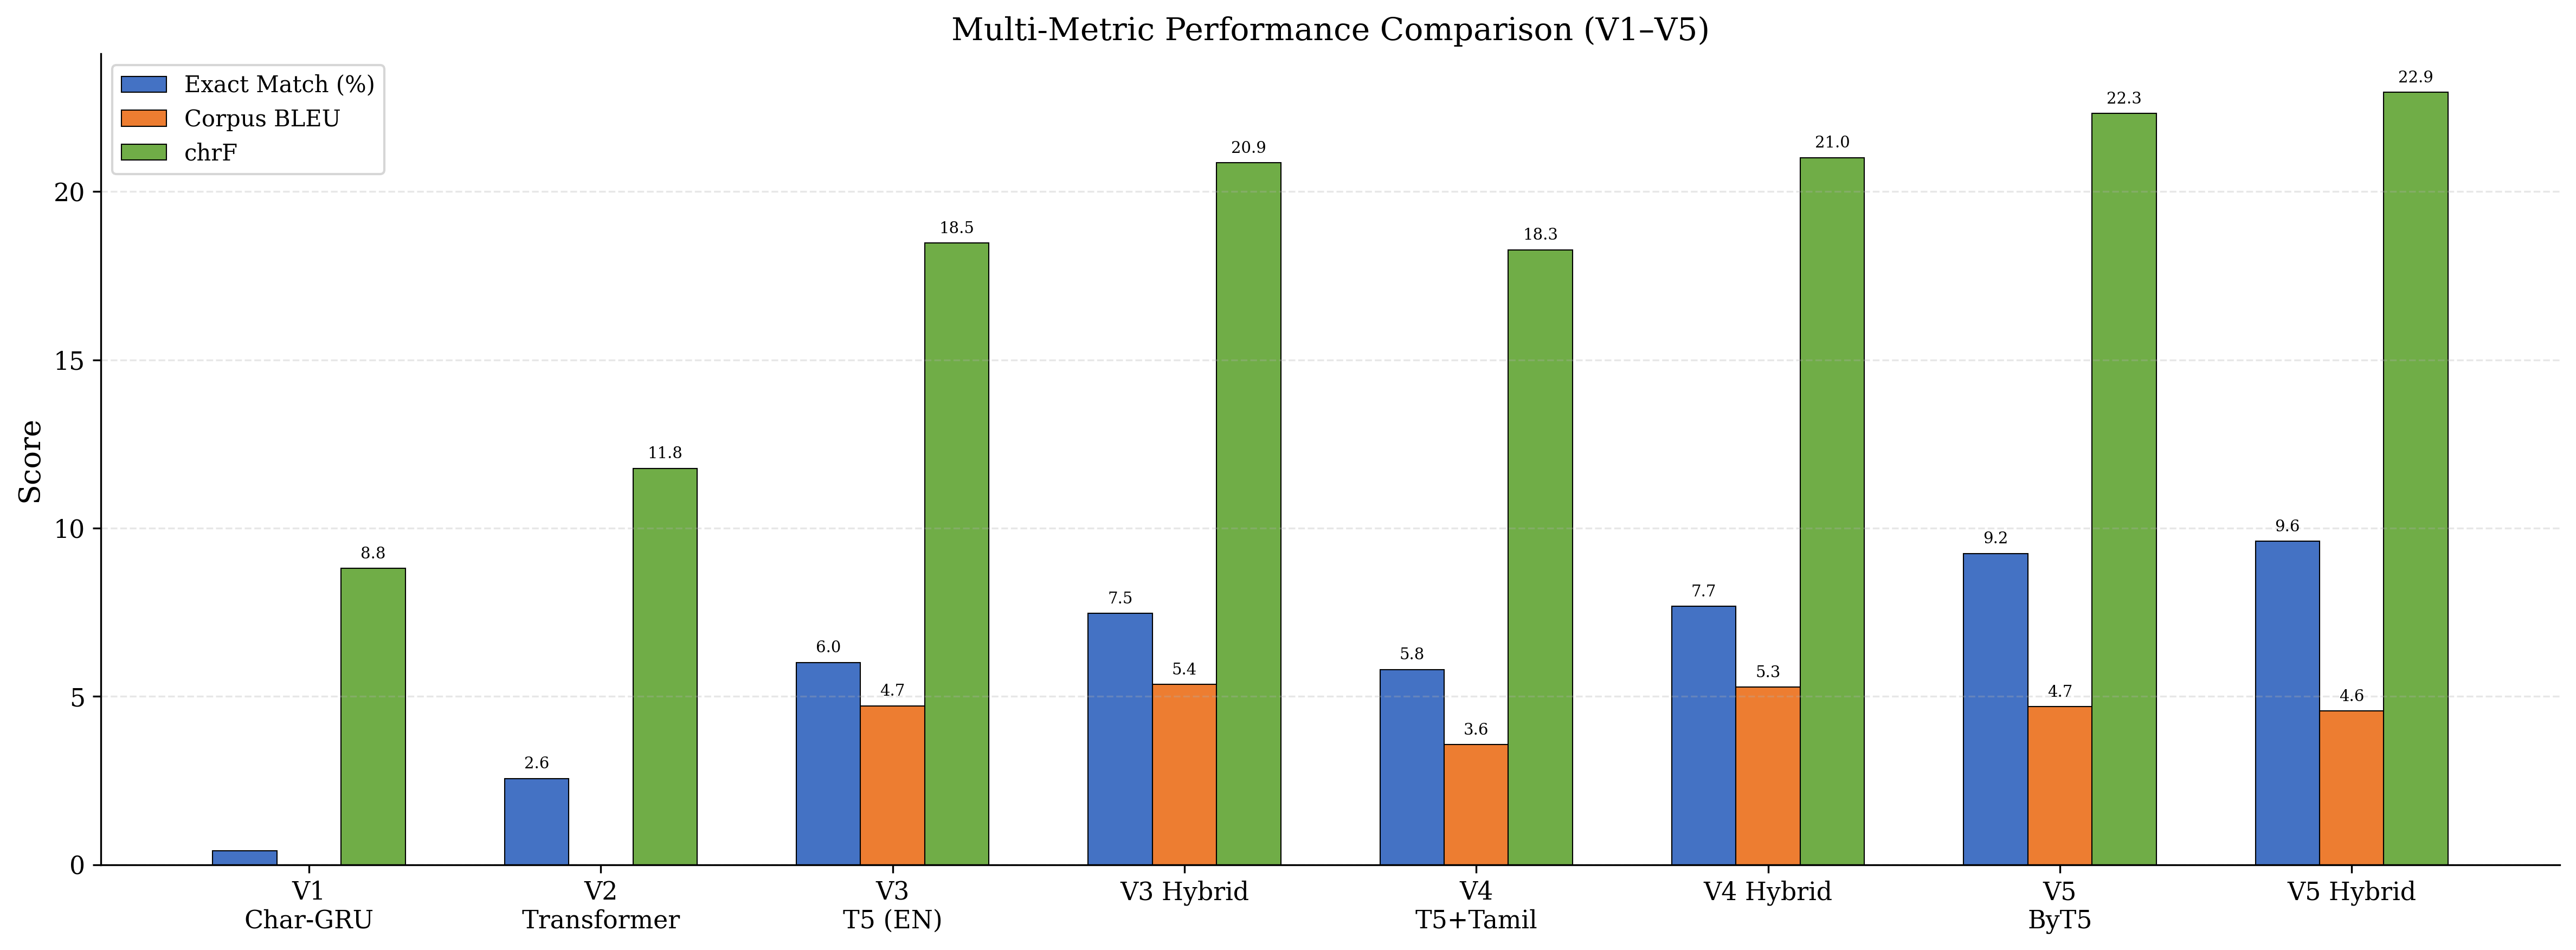
\includegraphics[width=\columnwidth]{fig2_multi_metric_comparison.png}}
\caption{Multi-metric performance comparison (EM, BLEU, chrF) across all model versions(V1-V5).}
\label{fig:multi_metric}
\end{figure}

\subsection{Training Dynamics}

The training loss curves established by all five model generations are as shown in Figure.~\ref{fig:loss_curves}. The training loss of V1 and V2 models reaches its highest point, as their modeling capacity has not yet developed enough. The training loss of V3 and V4, which is based on the T5 model, has a smaller training loss plateau compared to other models. The training loss of the V5 model is the lowest compared to all models, as its parameter capacity and byte-level tokenization advantages help in modeling the inputs better.


\begin{figure}[htbp]
\centerline{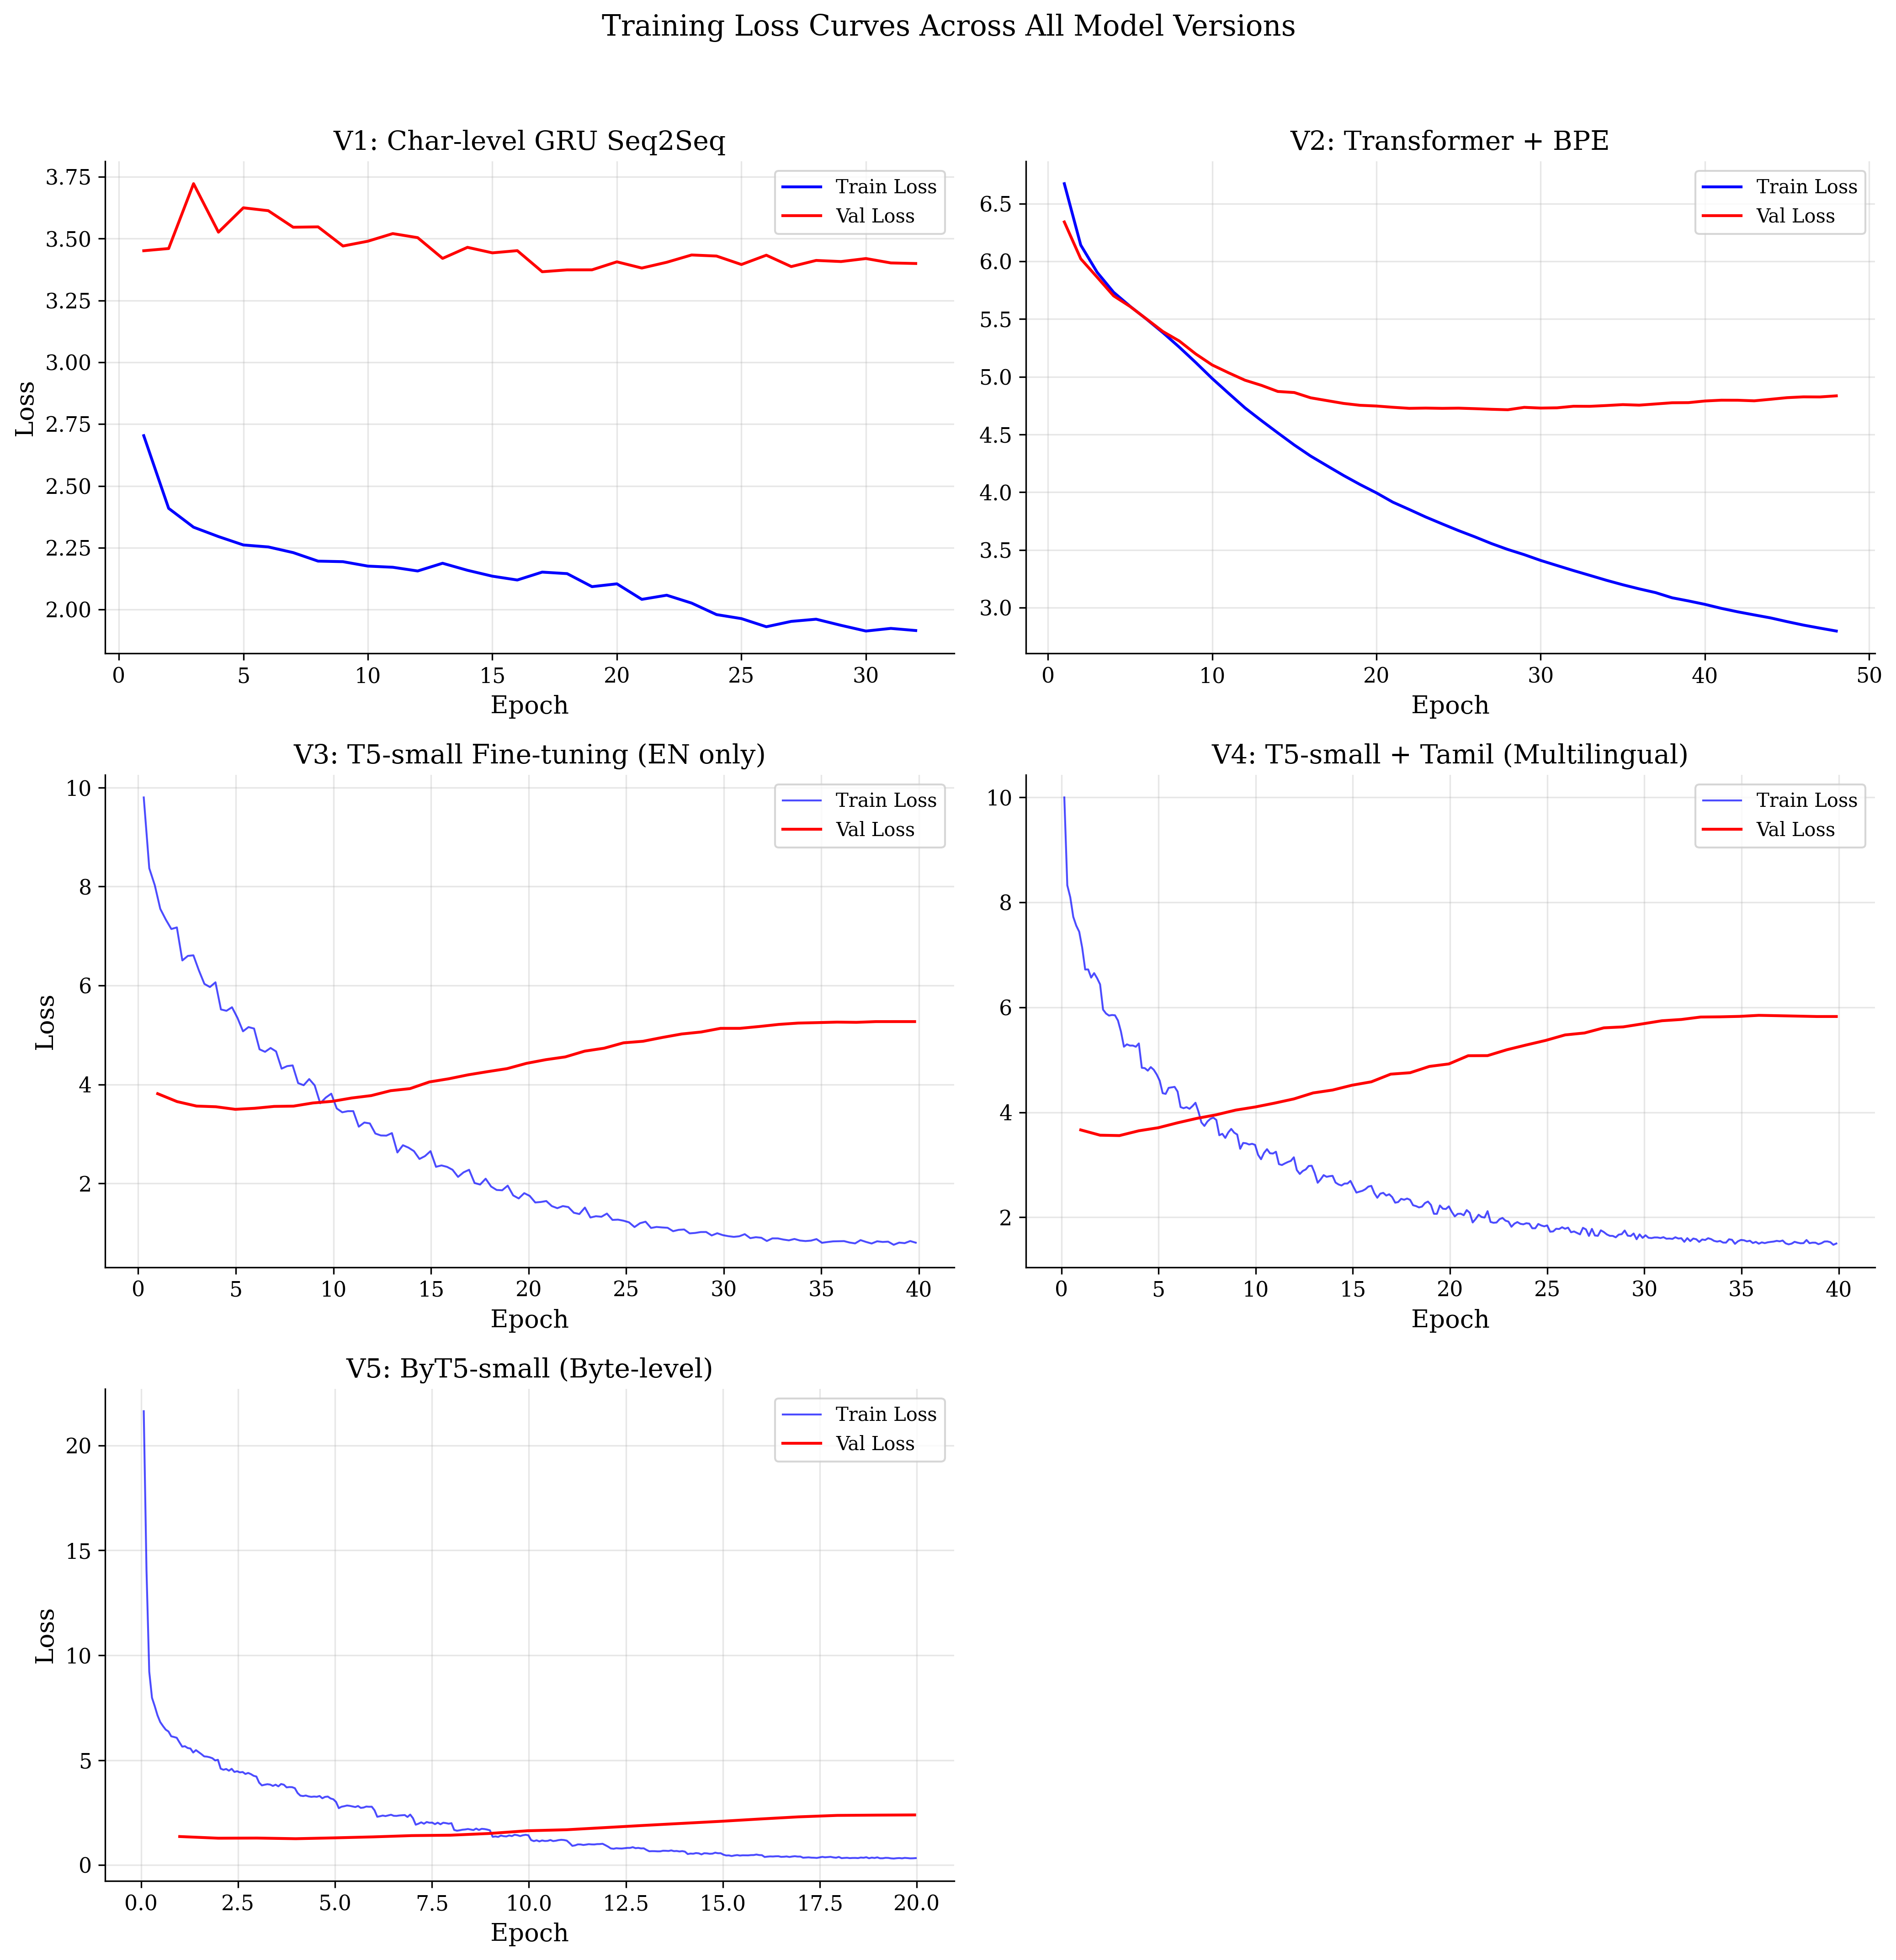
\includegraphics[width=\columnwidth]{fig3_training_loss_curves.png}}
\caption{Training loss curves for all 5 model generations(V1-V5).}
\label{fig:loss_curves}
\end{figure}

\subsection{Validation EM Progression}

Fig.~\ref{fig:em_progression} shows The exact match accuracy of the V3, V4, and V5 validation was obtained through multiple independent training runs, ensuring the results were reliable. The V5 system has the best initial development of all the models, which continues throughout the entire training process of 20 epochs. The model has better performance because the longer training time allows the system to produce better results through further optimization.

\begin{figure}[htbp]
\centerline{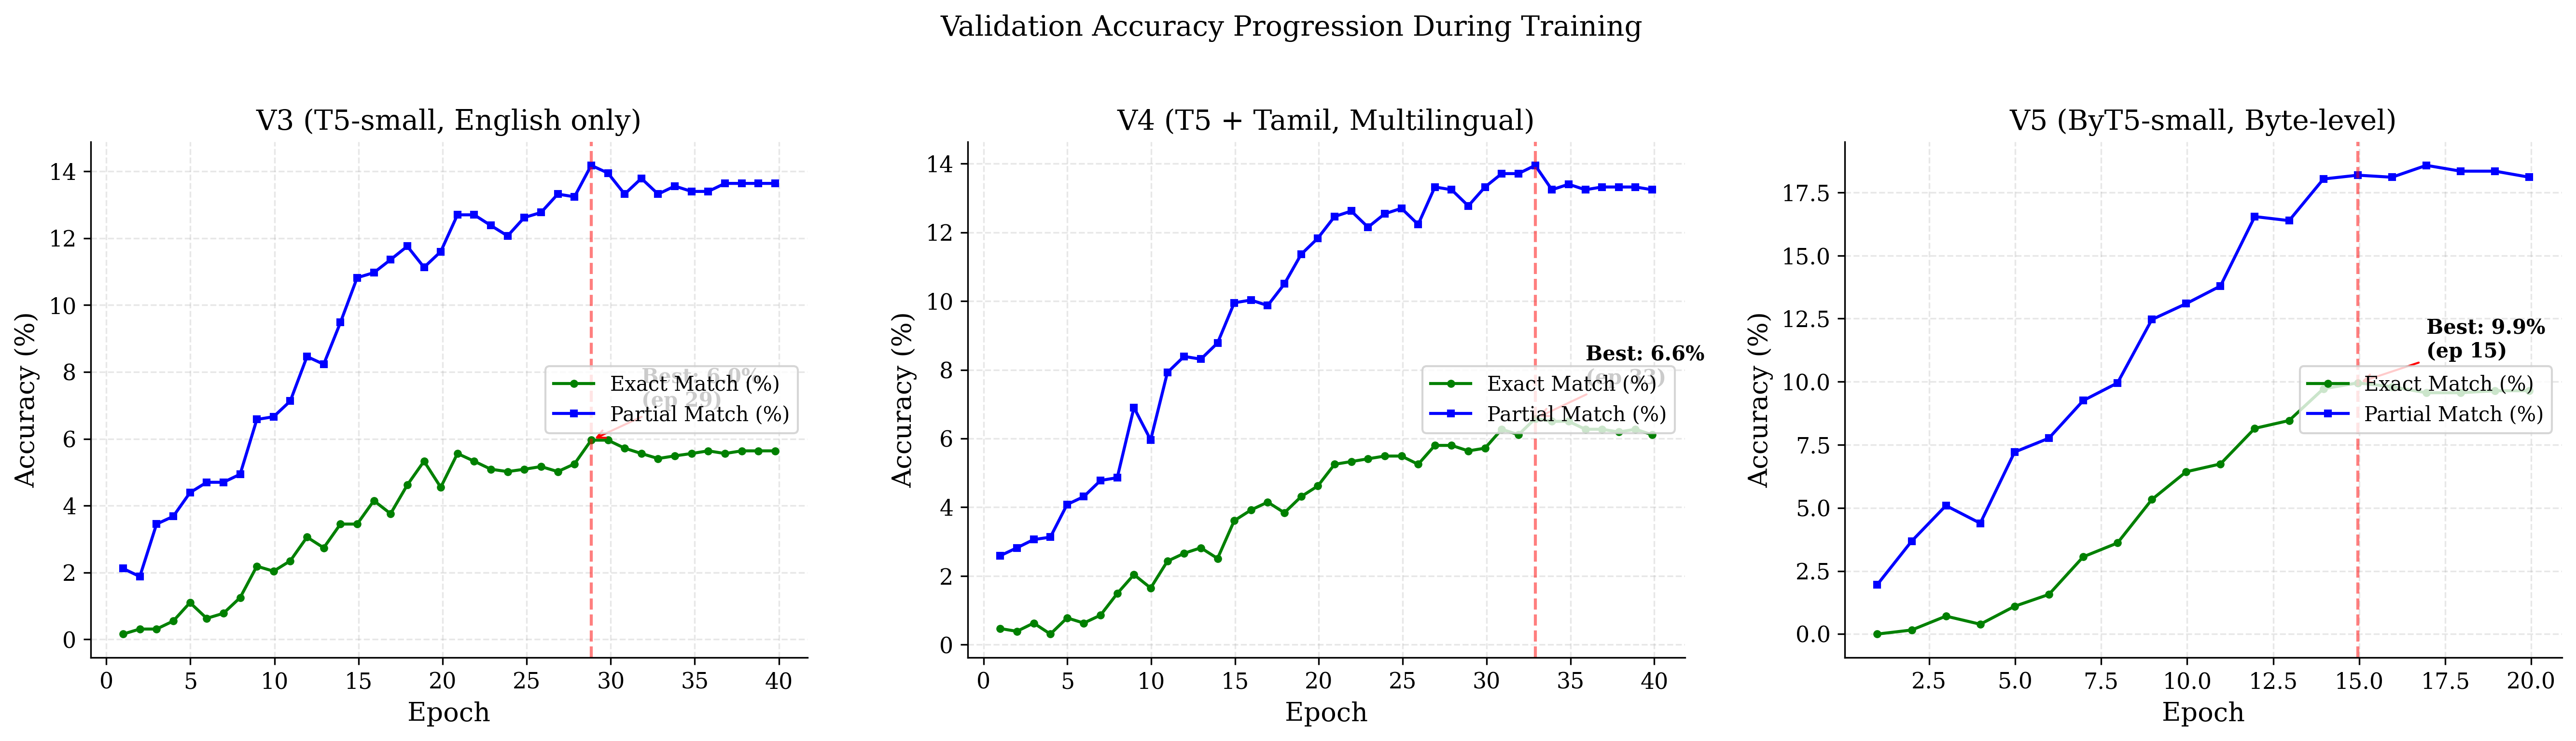
\includegraphics[width=\columnwidth]{fig4_v3_v4_v5_em_progression.png}}
\caption{Validation exact-match accuracy over training epochs (V3, V4, V5).}
\label{fig:em_progression}
\end{figure}

\subsection{Hybrid System Analysis}

The neural component and retrieval component of the respective hybrid systems contribute accordingly based on the data provided in Fig.~\ref{fig:hybrid_analysis}. The contribution of the V3 Hybrid system and the V4 Hybrid system in producing the right predictions comes from the fact that they utilize the retrieval method primarily in order to obtain the right predictions. The contribution of the V5 Hybrid system comes from the fact that it now operates based on a new distribution of predictions as the neural model takes control of 75.9\% of the predictions while showing better performance compared to all the previous hybrid systems.

\begin{figure}[htbp]
\centerline{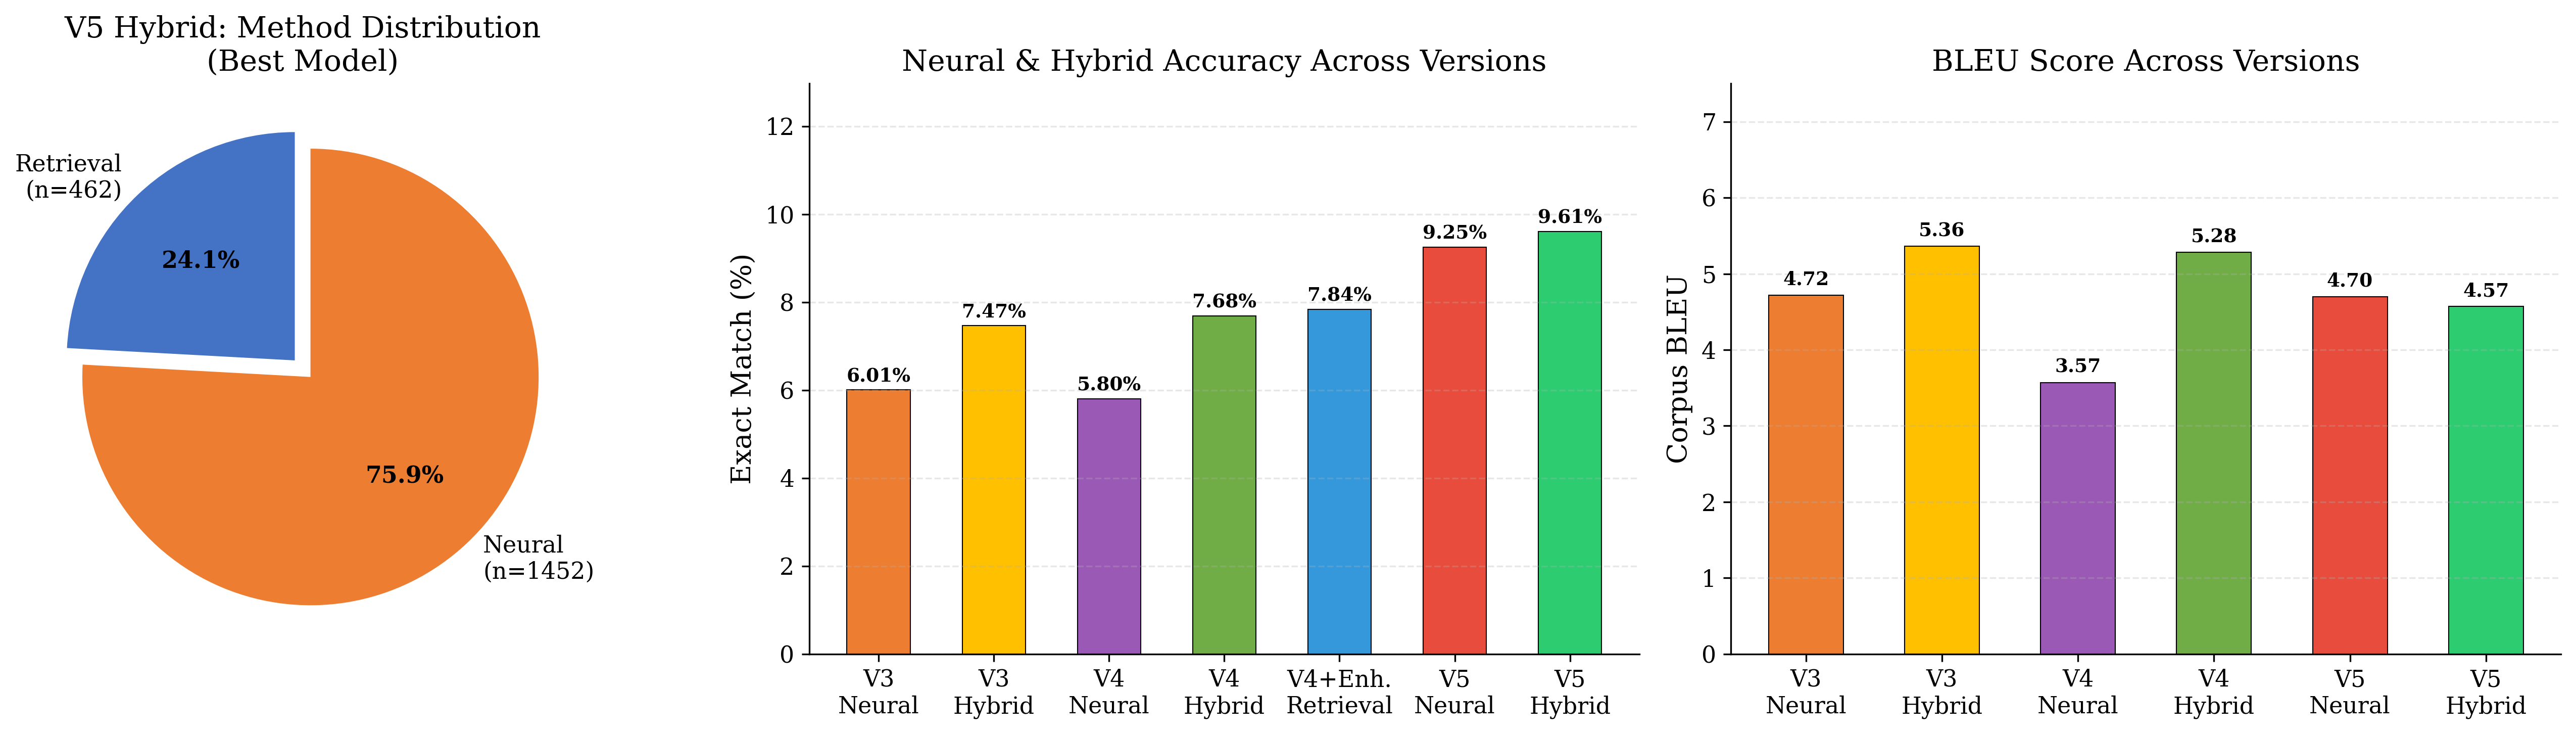
\includegraphics[width=\columnwidth]{fig5_hybrid_analysis.png}}
\caption{The Role of neural vs.\ retrieval components in each Hybrid Model.}
\label{fig:hybrid_analysis}
\end{figure}

\subsection{Category-Level Performance}

The accuracy of the results obtained in the study is presented in the semantic category analysis, which is depicted in Fig.~\ref{fig:category}. The concrete categories \textit{Animals},\textit{Colors}, and \textit{Kinship}, which people use in everyday life, produce higher accuracy results than the abstract categories \textit{Compound Verbs} and \textit{Concepts}. This is true in both V3 and V4 and V5.

\begin{figure}[htbp]
\centerline{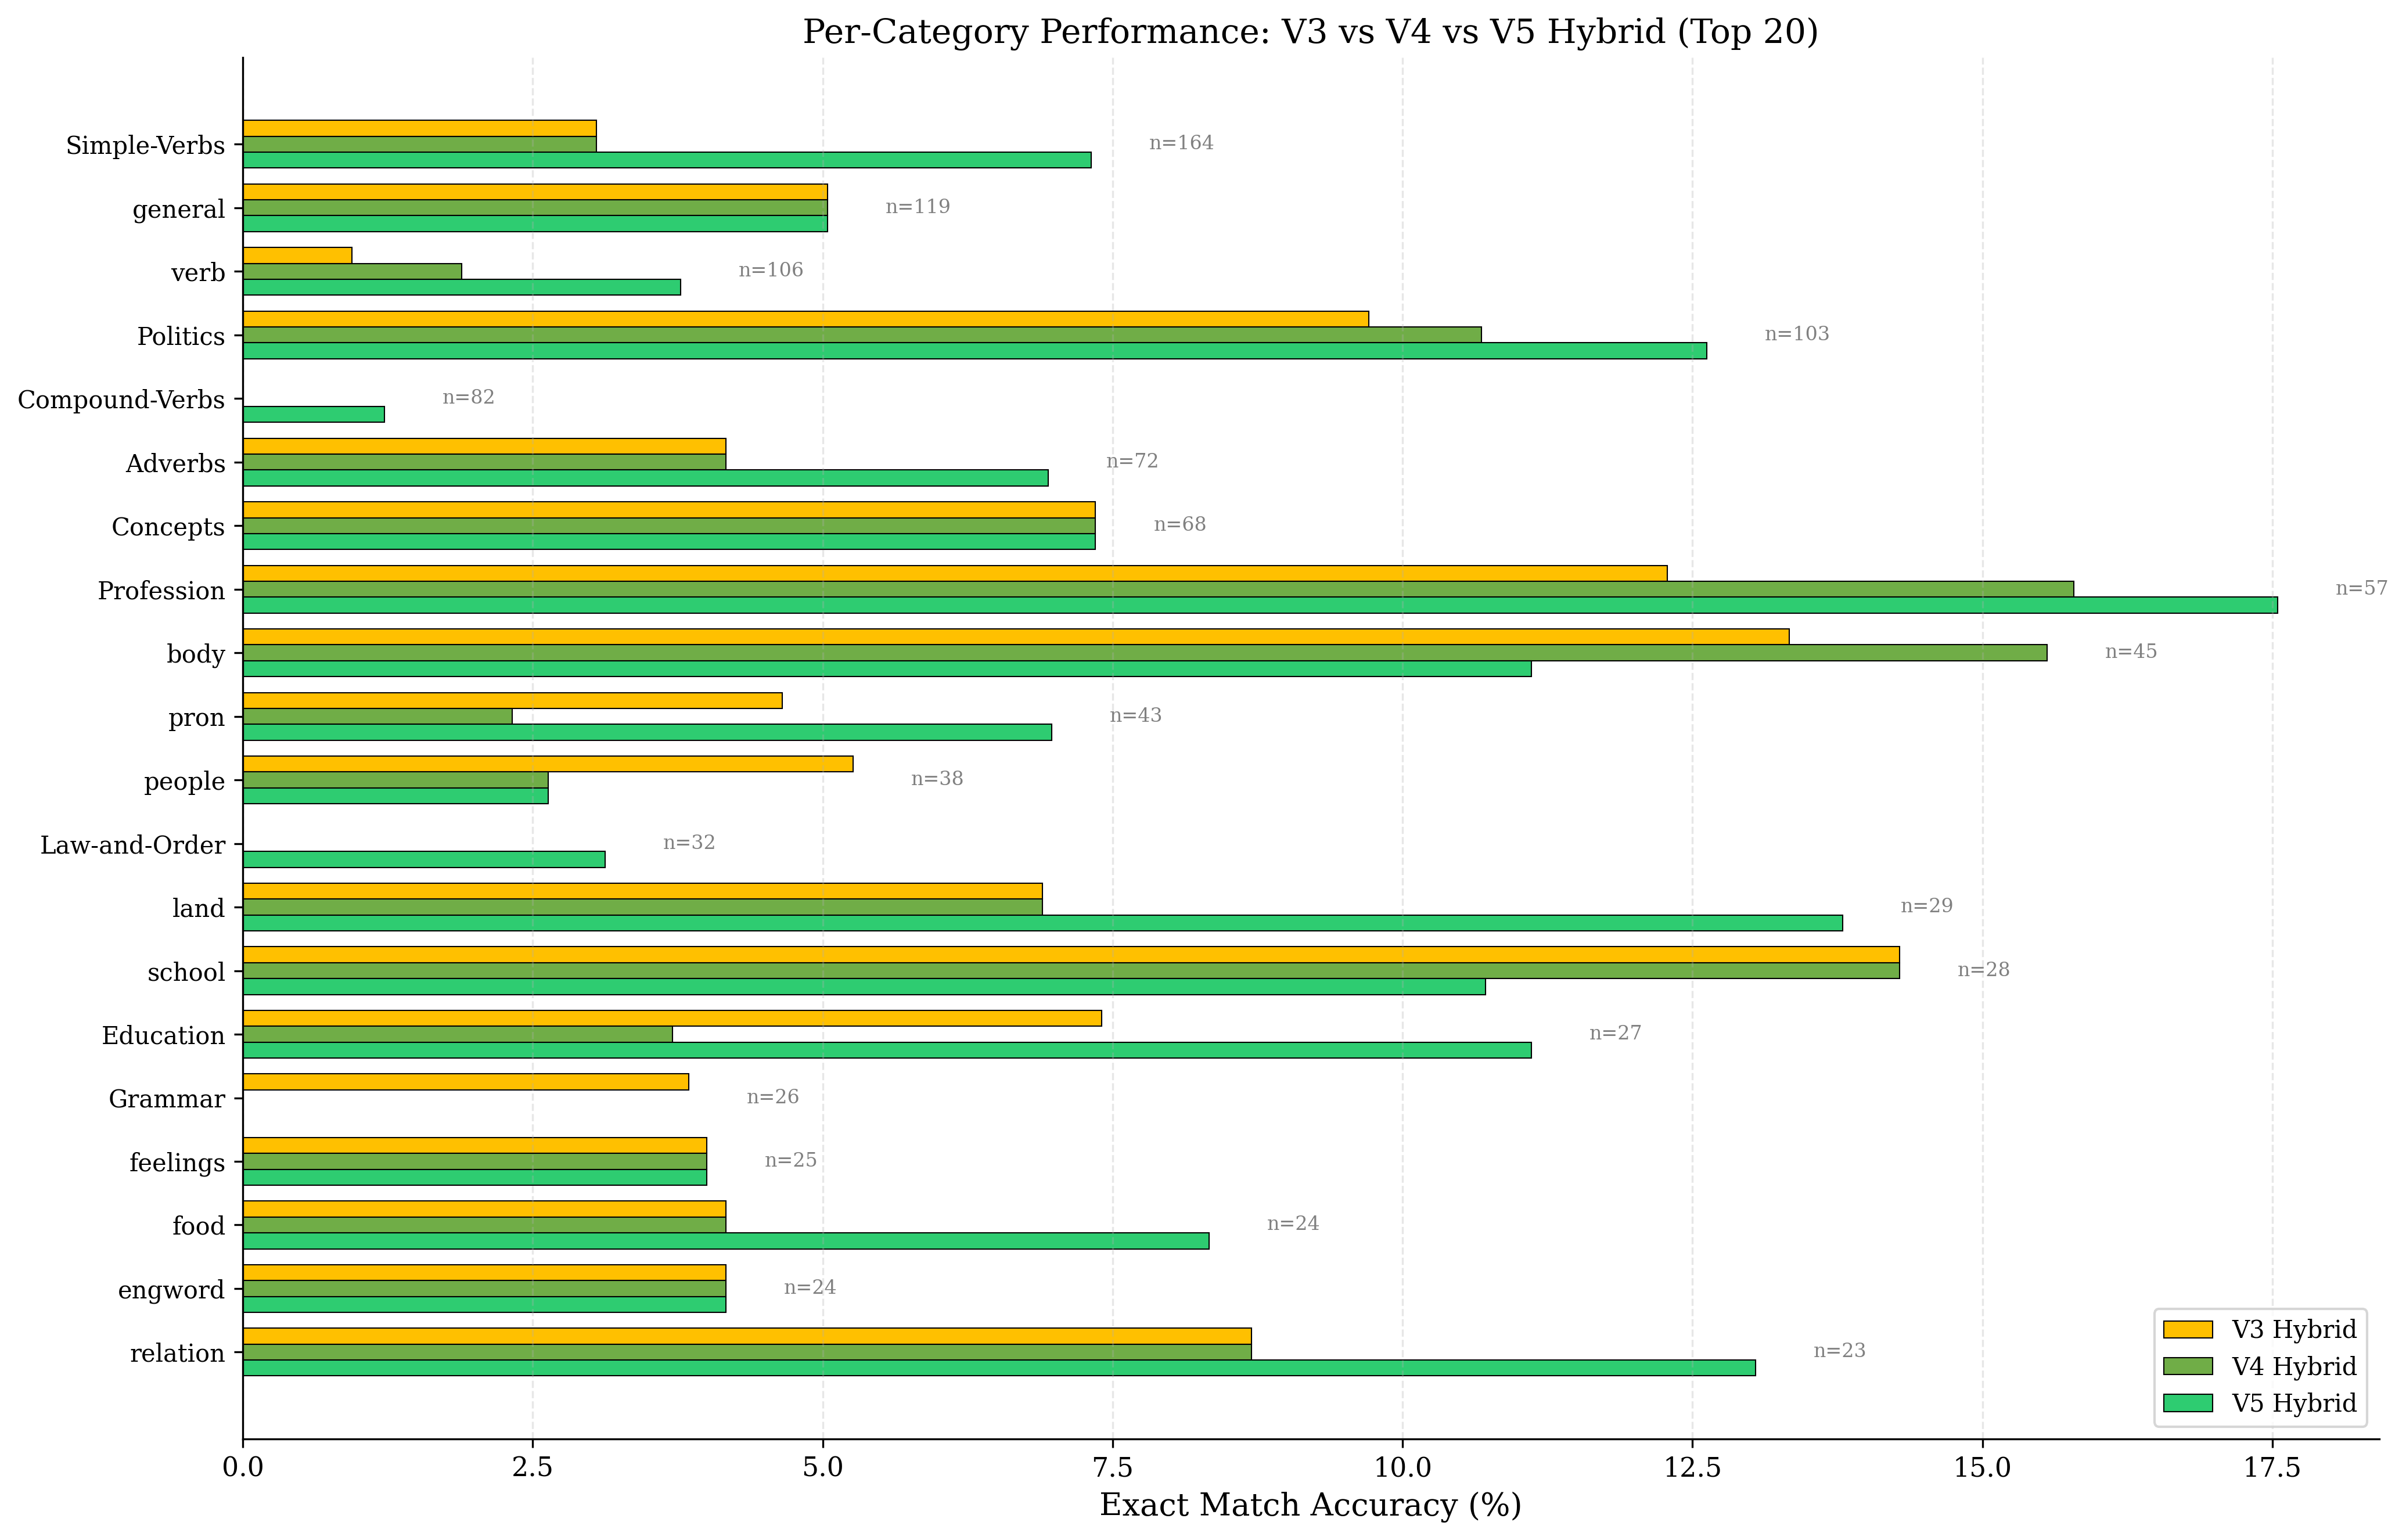
\includegraphics[width=\columnwidth]{fig6_category_performance.png}}
\caption{Per-category exact-match accuracy for V3, V4, and V5 (top categories).}
\label{fig:category}
\end{figure}

\subsection{Improvement Timeline}

The graph in Fig.~\ref{fig:timeline} presents the total development progress from the first version until the fifth version of the Hybrid system. The architectural changes in the system's development included the change from character encoding to subword encoding, from scratch training to the use of pre-trained models, and from subword to byte-level processing, as well as the change from pure neural systems to the use of hybrid systems. The total system improvement was 22.9$\times$.


\begin{figure}[htbp]
\centerline{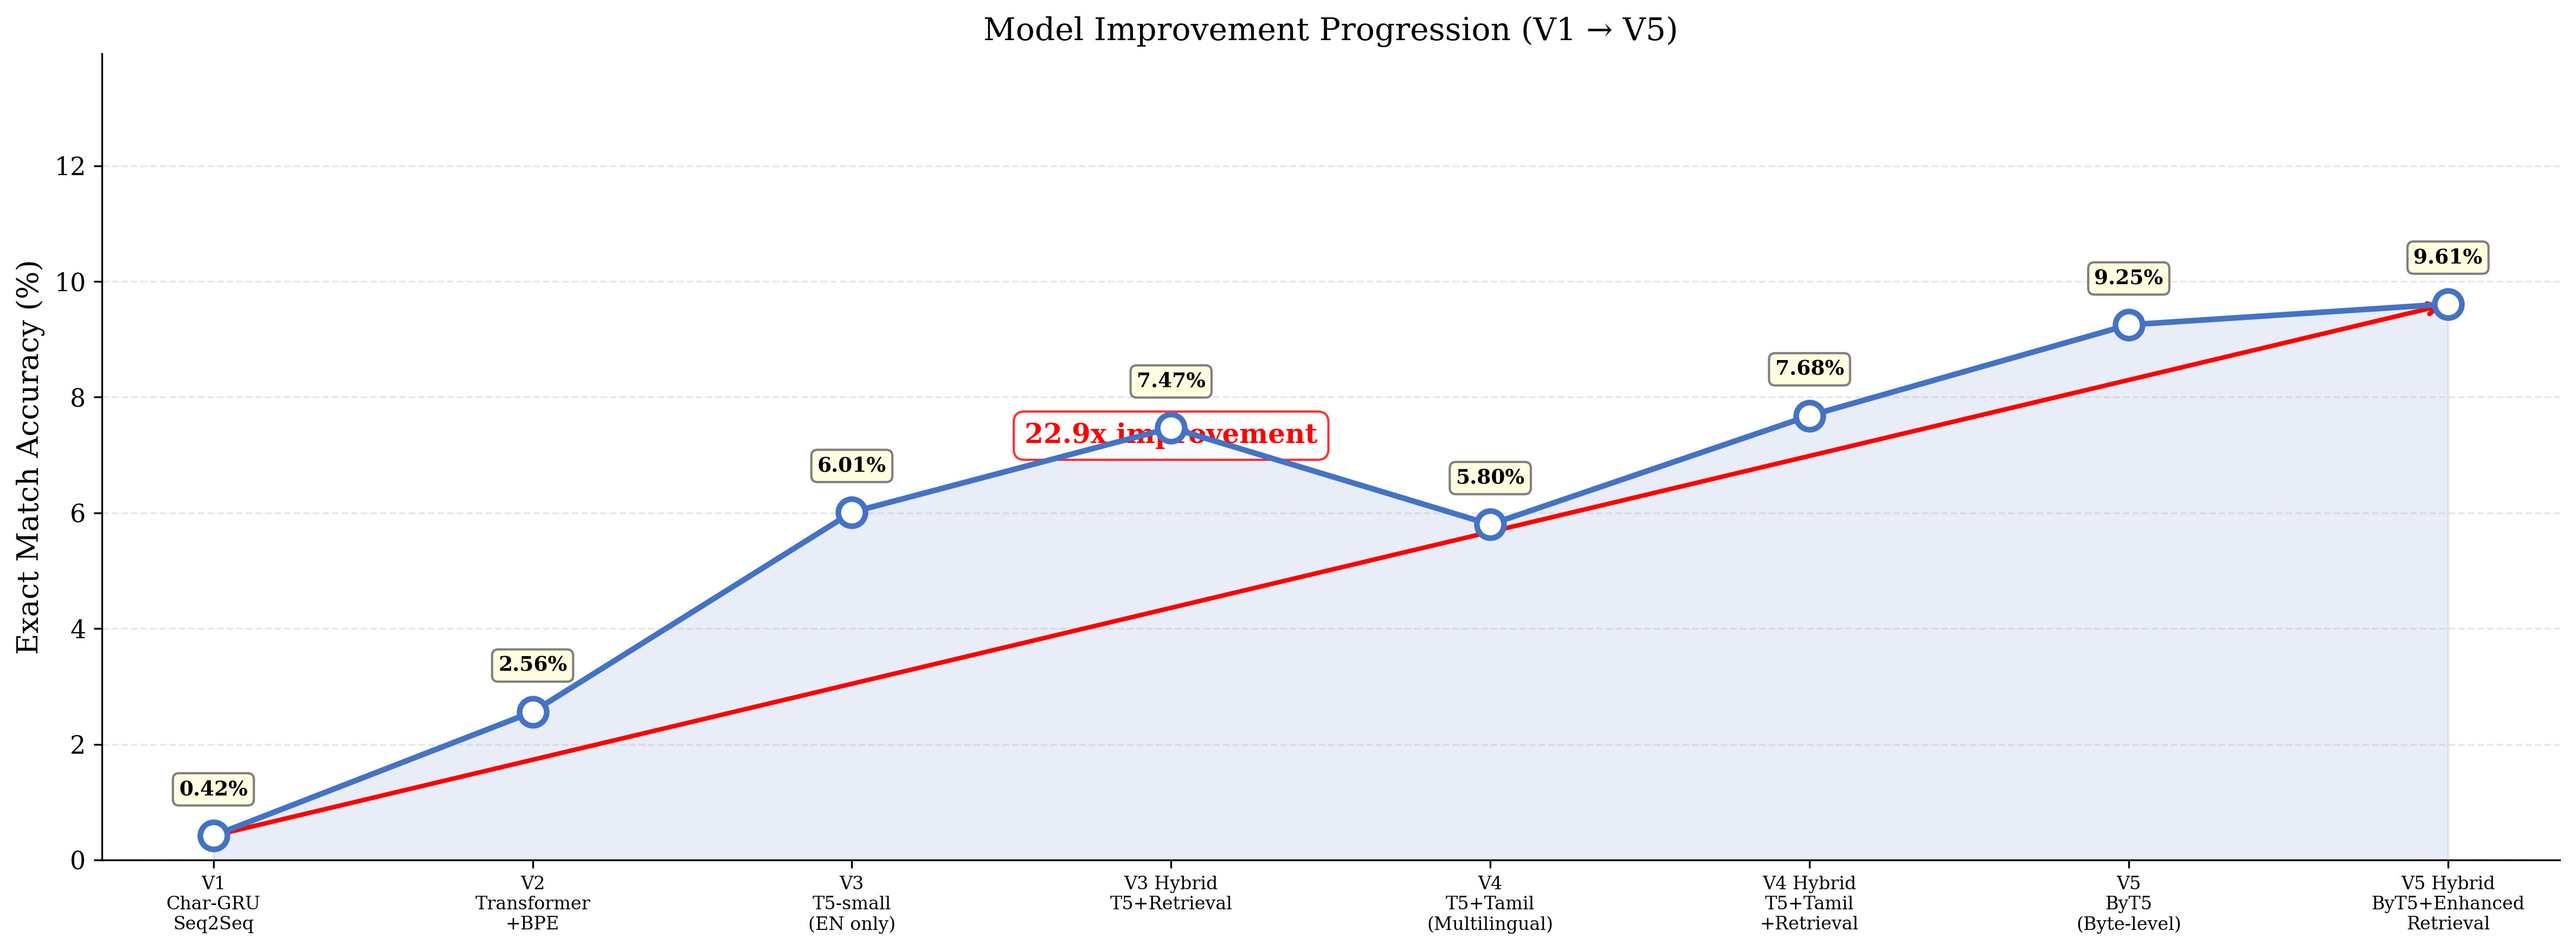
\includegraphics[width=\columnwidth]{fig9_improvement_progression.png}}
\caption{Increase in the figure of exact-match scores reached (22.9$\times$ total gain).the improvement of the global data from V1 to V5 Hybrid.}
\label{fig:timeline}
\end{figure}

\subsection{Qualitative Analysis}

Table~\ref{tab:examples} shows prediction samples that were generated by the V5 neural model. The prediction samples illustrate the ability of the system to process various types of semantic information. The semantic understanding of the model is demonstrated by its ability to show that it can recognize various meanings. The model is able to successfully predict the input value based on the reference to "greatness/superiority" because it has an understanding of its meaning.

\begin{table}[htbp]
\centering
\caption{Example V5 Neural Predictions}
\label{tab:examples}
\begin{tabular}{llll}
\toprule
\textbf{Source} & \textbf{Reference} & \textbf{Prediction} & \textbf{Cat.} \\
\midrule
mhaLi & Fish & Fish \checkmark & animal \\
phalti phaar & morning & morning \checkmark & Time \\
thanait & policeman & policeman \checkmark & Prof. \\
chakravarti & emperor & emperor \checkmark & Politics \\
sulo & Winnow. basket & Winnow. basket \checkmark & kitchen \\
dairo & Left & Left \checkmark & opp \\
\midrule
pirEv pOT & Like & Love & verb \\
angam & organ & thigh & Body \\
poshaan & Corridor & Address & house \\
\bottomrule
\end{tabular}
\end{table}

\subsection{Error Analysis}

The 1737 predictions made by the V5 Neural system were analyzed to identify the three different types of errors that were made. The first type of error that includes \textit{synonym substitution} amounts to 7\% of the total errors made by the system because it produces a valid translation that is not the correct reference string (e.g., “beautifully” as opposed to “fairly, beautifully”). The second type of error that amounts to 32\% of the errors made is where the prediction is made based on a \textit{semantic concept} that is contained within the correct meaning range but has a word that sounds similar to the correct answer (e.g., “thigh” as opposed to “organ”). The final 61\% of the results are from the unrelated output that mostly includes uncommon vocabulary items that are contained in limited training resources.

\begin{figure}[htbp]
\centerline{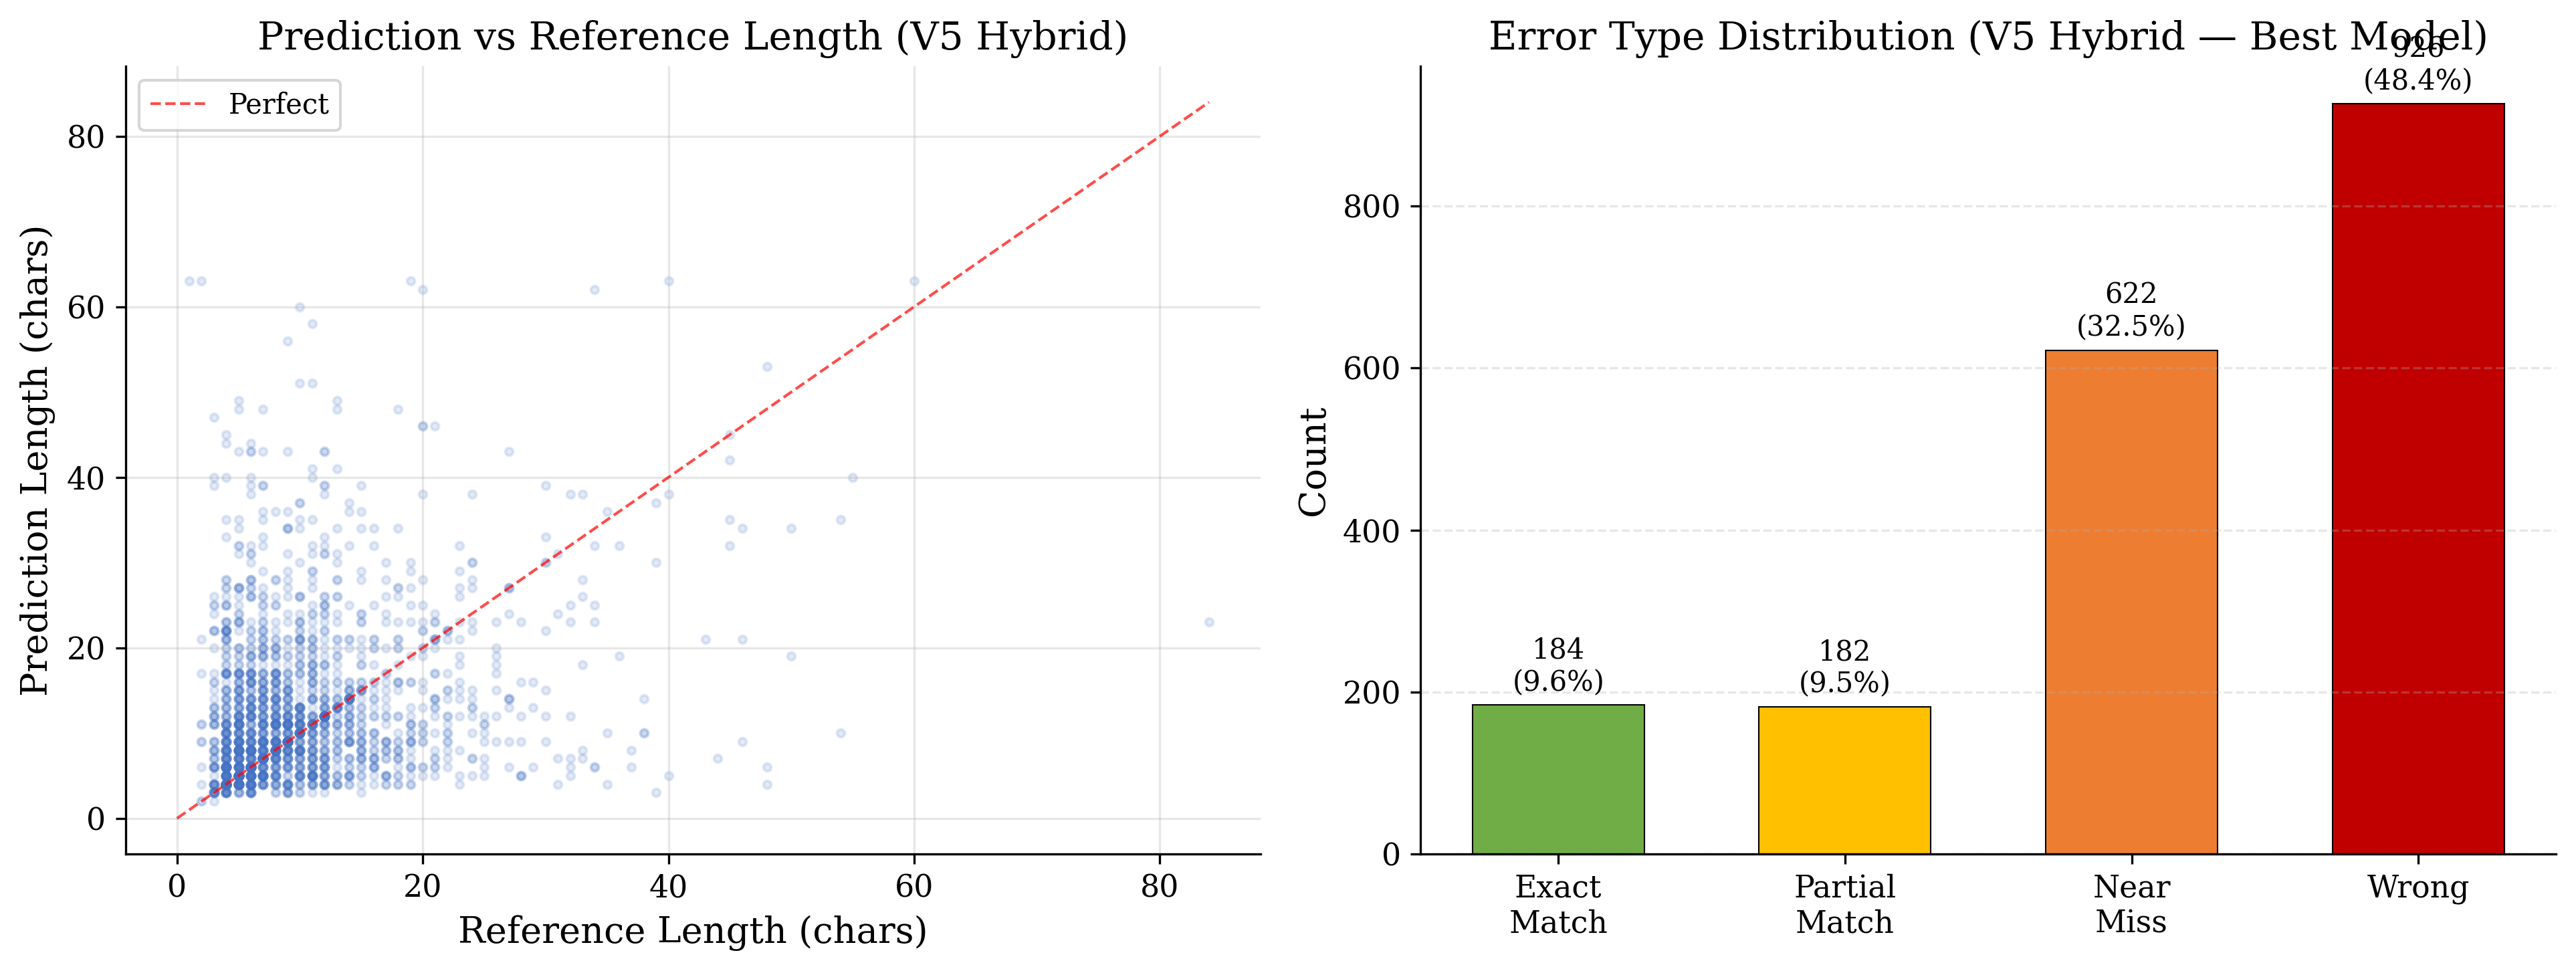
\includegraphics[width=\columnwidth]{fig8_error_analysis.png}}
\caption{Error type distribution for V5 Hybrid Model predictions.}
\label{fig:error_analysis}
\end{figure}

% ═══════════════════════════════════════════════════════════
\section{Web Application}\label{sec:webapp}
% ═══════════════════════════════════════════════════════════

The research team developed a web application that allows users to search for dictionary entries in the Sourashtra dictionary with the help of the user's preferred input language, English or Tamil. The web application works on the basis of processing the queries entered by the users in their preferred language, English and Tamil, to retrieve the dictionary entries from the dictionary database containing 12758 entries and provide the corresponding word in the Sourashtra language with its original script. The system design allows more users to access the system while the system maintains its original linguistic features.

\subsection{Architecture}

The backend system uses a lightweight server based on the Flask framework, which loads the dictionary data into memory during startup to build lowercase character arrays and character n-gram sets that facilitate fast similarity search. The retrieval function uses the three-signal scoring formula presented in Eq.~\ref{eq:retrieval}. The system sends back the results in JSON format, which the client-side JavaScript interface uses to display the data.

\subsection{Sourashtra Script Rendering}

The interface needed to display the results in the form of the Saurashtra script. The reason for this is that the original Saurashtra script was needed to display the results. We have used Google Noto Sans Saurashtra as the web font for our application because it has precise font rendering. The user interface displays each result card that has the Sourashtra script as the major component and displays the Romanized transliteration with English or Tamil translation as secondary information.

\subsection{User Interface}

The system has three major interactive views that can be used to interact with the system. Anyone can type a word and view the results instantly by clicking on the “Translate” tab. The Dictionary tab allows the user to browse through all the 12,758 entries while the user searches and filters the entries. The About tab shows a summary of the project, including how the models have changed over the time and a little information on the Sourashtra script.

\begin{figure}[htbp]
\centerline{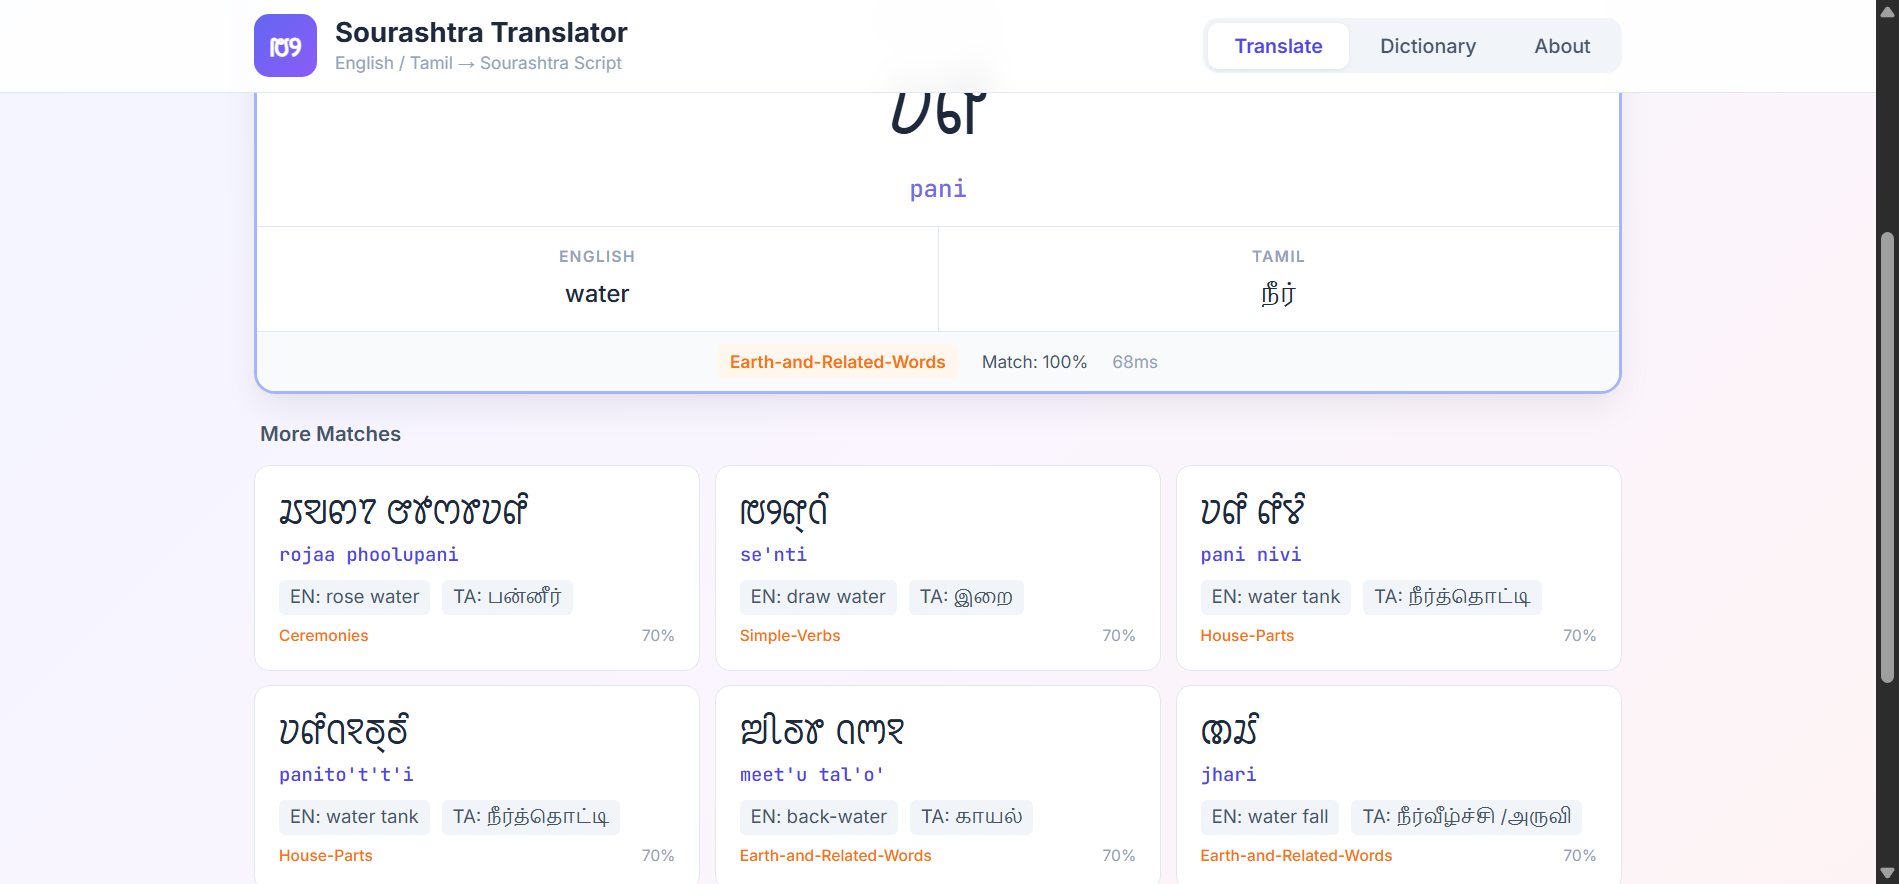
\includegraphics[width=\columnwidth]{webapp_translate.png}}
\caption{Web application: Main page showing a query request result with native Sourashtra script output.}
\label{fig:webapp_translate}
\end{figure}

\begin{figure}[htbp]
\centerline{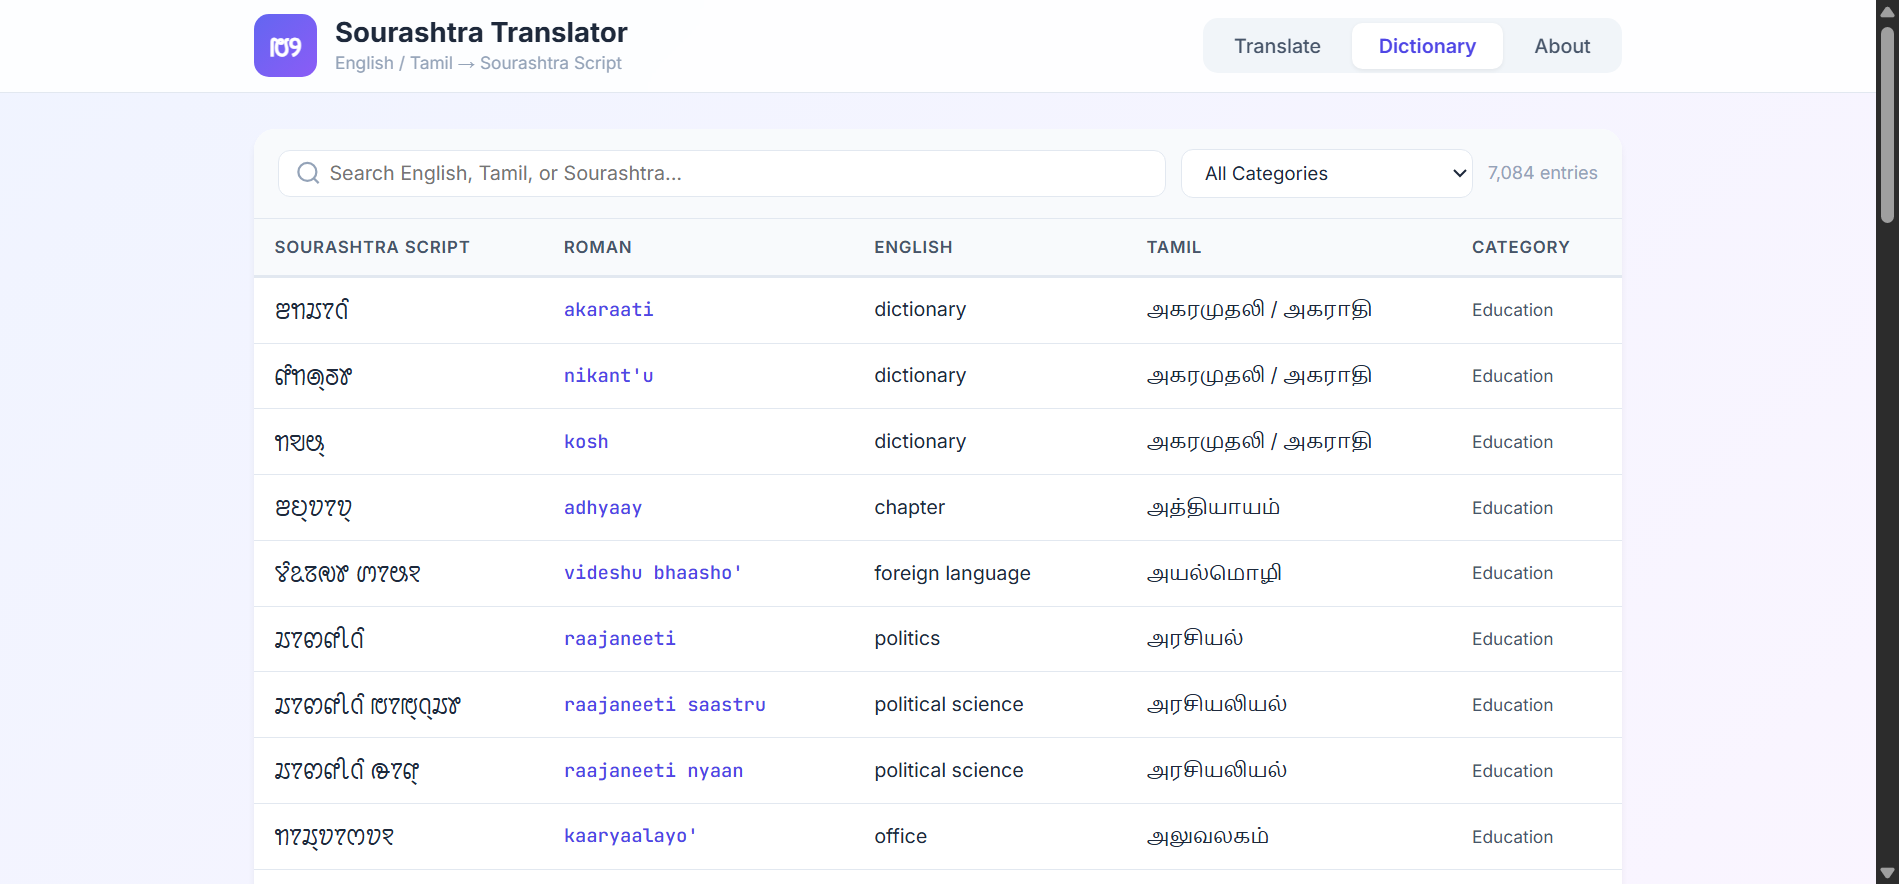
\includegraphics[width=\columnwidth]{webapp_dictionary.png}}
\caption{Web application: Dictionary page with search and category filter for the reference.}
\label{fig:webapp_dictionary}
\end{figure}

% ═══════════════════════════════════════════════════════════
\section{Discussion}
% ═══════════════════════════════════════════════════════════

The research has revealed that the neural machine translation technology has been beneficial to extremely low-resource languages, but the current state of the system requires further improvements to enable it to work entirely. Although the exact match accuracy of 9.61\% in the translation system of high-resource languages is very low, it is a real step forward since the ability did not exist in the field before the accomplishment.

The system has some limitations in performance since several factors exist, and the \textbf{size of the data} is the primary constraint in the performance of the system. The training process of the model requires 9,568 base training pairs, which limits the ability of the system to learn knowledge about various lexical items and morphological structures. The system does not fully comprehend the Sourashtra language since it does not have the ability to process all the structures of the language, which limits the ability to produce accurate translation results.

\textbf{Word-level evaluation.} The data set provided includes word pairs, which indicate how words relate to each other but not sentences. The testing process is made harder by the fact that any change in the characters will cause a failure in the test. The two metrics, BLEU and chrF, offer precise measurements for evaluation of the text provided.

\textbf{One-to-many mappings.}There are multiple English translations for each of the Sourashtra words. The two words, "close, cover" and "Dissolve, Melt," indicate that there are multiple English translations for Sourashtra words. The system recognizes all word translations, but our system only recognizes a single string. The evaluation system, which recognizes all word translations, will lead to better accuracy results.

\textbf{Script complexity.} The Saurashtra script is an abugida with non-trivial vowel-sign combinations, making romanization schemes inconsistent and introducing noise in the source data.

Despite these challenges, the progressive approach proved valuable. Each generation taught us something that informed the next: V1 showed that character-level models cannot bridge the script gap; V2 demonstrated the benefit of attention and subwords; V3 proved that pre-training compensates for small data; V4 revealed that cross-lingual transfer requires tokenizer compatibility; and V5 validated the byte-level hypothesis.

% ═══════════════════════════════════════════════════════════
\section{Conclusion and Future Work}\label{sec:conclusion}
% ═══════════════════════════════════════════════════════════

We have presented a progressive approach to building a neural machine translation system for Sourashtra, an endangered Indo-Aryan language with extremely limited parallel data. Starting from a character-level GRU baseline achieving 0.42\% exact-match accuracy, we improved performance 22.9-fold to 9.61\% through a series of architectural advances: subword tokenization, pre-trained Transformer fine-tuning, cross-lingual transfer with Tamil, byte-level modeling with ByT5, and hybrid neural-retrieval inference.

Several directions remain for future work. Back-translation could generate synthetic parallel data to expand the training corpus. Training on larger byte-level models (e.g., ByT5-base or mT5-large) with more compute resources may push accuracy further. Sentence-level translation, rather than word-level, would better test the system's ability to handle morphology and syntax. Community involvement could yield additional parallel text, including conversational data, religious texts, and folk literature. Finally, extending the web application to support bidirectional translation---both English/Tamil$\rightarrow$Sourashtra and Sourashtra$\rightarrow$English---with the neural model would create a practical tool for language learners and community members working to preserve this endangered language.

\section*{Acknowledgment}

We thank the Sourashtra community and the maintainers of the open-source Sourashtra dictionary project for making the parallel data used in this research freely available.

\begin{thebibliography}{00}

\bibitem{vaswani2017attention}
A.~Vaswani, N.~Shazeer, N.~Parmar, J.~Uszkoreit, L.~Jones, A.~N.~Gomez, \L.~Kaiser, and I.~Polosukhin, ``Attention is all you need,'' in \textit{Advances in Neural Information Processing Systems}, vol.~30, 2017, pp.~5998--6008.

\bibitem{ethnologue2023}
D.~M.~Eberhard, G.~F.~Simons, and C.~D.~Fennig, Eds., \textit{Ethnologue: Languages of the World}, 26th ed. Dallas, TX: SIL International, 2023. [Online]. Available: \url{https://www.ethnologue.com}

\bibitem{sourashtra_dict}
Sourashtra Community Dictionary Project, ``Open-source Sourashtra-English-Tamil dictionary,'' GitHub repository, 2023.

\bibitem{bahdanau2015attention}
D.~Bahdanau, K.~Cho, and Y.~Bengio, ``Neural machine translation by jointly learning to align and translate,'' in \textit{Proc.\ 3rd Int.\ Conf.\ Learning Representations (ICLR)}, 2015.

\bibitem{sennrich2016bpe}
R.~Sennrich, B.~Haddow, and A.~Birch, ``Neural machine translation of rare words with subword units,'' in \textit{Proc.\ 54th Annu.\ Meeting Assoc.\ Comput.\ Linguistics (ACL)}, 2016, pp.~1715--1725.

\bibitem{sennrich2016backtranslation}
R.~Sennrich, B.~Haddow, and A.~Birch, ``Improving neural machine translation models with monolingual data,'' in \textit{Proc.\ 54th Annu.\ Meeting Assoc.\ Comput.\ Linguistics (ACL)}, 2016, pp.~86--96.

\bibitem{kudo2018sentencepiece}
T.~Kudo and J.~Richardson, ``SentencePiece: A simple and language independent subword tokenizer and detokenizer for neural text processing,'' in \textit{Proc.\ Conf.\ Empirical Methods Natural Language Processing (EMNLP): System Demonstrations}, 2018, pp.~66--71.

\bibitem{raffel2020t5}
C.~Raffel, N.~Shazeer, A.~Roberts, K.~Lee, S.~Narang, M.~Matena, Y.~Zhou, W.~Li, and P.~J.~Liu, ``Exploring the limits of transfer learning with a unified text-to-text Transformer,'' \textit{J.\ Machine Learning Research}, vol.~21, no.~140, pp.~1--67, 2020.

\bibitem{xue2022byt5}
L.~Xue, A.~Barua, N.~Constant, R.~Al-Rfou, S.~Narang, M.~Kale, A.~Roberts, and C.~Raffel, ``ByT5: Towards a token-free future with pre-trained byte-to-byte models,'' \textit{Trans.\ Assoc.\ Comput.\ Linguistics}, vol.~10, pp.~291--306, 2022.

\bibitem{xue2021mt5}
L.~Xue, N.~Constant, A.~Roberts, M.~Kale, R.~Al-Rfou, A.~Siddhant, A.~Barua, and C.~Raffel, ``mT5: A massively multilingual pre-trained text-to-text Transformer,'' in \textit{Proc.\ 2021 Conf.\ North American Chapter Assoc.\ Comput.\ Linguistics (NAACL)}, 2021, pp.~483--498.

\bibitem{liu2020mbart}
Y.~Liu \textit{et al.}, ``Multilingual denoising pre-training for neural machine translation,'' \textit{Trans.\ Assoc.\ Comput.\ Linguistics}, vol.~8, pp.~726--742, 2020.

\bibitem{zoph2016transfer}
B.~Zoph, D.~Yuret, J.~May, and K.~Knight, ``Transfer learning for low-resource neural machine translation,'' in \textit{Proc.\ Conf.\ Empirical Methods Natural Language Processing (EMNLP)}, 2016, pp.~1568--1575.

\bibitem{neubig2018rapid}
G.~Neubig and J.~Hu, ``Rapid adaptation of neural machine translation to new languages,'' in \textit{Proc.\ Conf.\ Empirical Methods Natural Language Processing (EMNLP)}, 2018, pp.~875--880.

\bibitem{lee2017fully}
J.~Lee, K.~Cho, and T.~Hofmann, ``Fully character-level neural machine translation without explicit segmentation,'' \textit{Trans.\ Assoc.\ Comput.\ Linguistics}, vol.~5, pp.~365--378, 2017.

\bibitem{foley2018building}
B.~Foley \textit{et al.}, ``Building speech recognition systems for language documentation: The CoEDL experience,'' in \textit{Proc.\ 6th Int.\ Conf.\ Language Documentation and Conservation (ICLDC)}, 2018.

\bibitem{micher2017improving}
J.~Micher, ``Improving coverage of an Inuktitut morphological analyzer using a segmental recurrent neural network,'' in \textit{Proc.\ 2nd Workshop on Computational Methods for Endangered Languages}, 2017.

\bibitem{dowling2020smt}
M.~Dowling, T.~Lynn, A.~Poncelas, and A.~Way, ``A large-scale study of the effectiveness of SMT and NMT for the translation of lesser-resourced language pairs,'' \textit{Machine Translation}, vol.~34, pp.~1--31, 2020.

\bibitem{papineni2002bleu}
K.~Papineni, S.~Roukos, T.~Ward, and W.~J.~Zhu, ``BLEU: A method for automatic evaluation of machine translation,'' in \textit{Proc.\ 40th Annu.\ Meeting Assoc.\ Comput.\ Linguistics (ACL)}, 2002, pp.~311--318.

\bibitem{popovic2015chrf}
M.~Popovi\'{c}, ``chrF: Character $n$-gram F-score for automatic MT evaluation,'' in \textit{Proc.\ 10th Workshop Statistical Machine Translation}, 2015, pp.~392--395.

\bibitem{wolf2020huggingface}
T.~Wolf \textit{et al.}, ``Transformers: State-of-the-art natural language processing,'' in \textit{Proc.\ Conf.\ Empirical Methods Natural Language Processing (EMNLP): System Demonstrations}, 2020, pp.~38--45.

\end{thebibliography}

\end{document}
